 %% ++++++++++++++++++++++++++++++++++++++++++++++++++++++++++++
%% Hauptdatei, Wurzel des Dokuments
%% ++++++++++++++++++++++++++++++++++++++++++++++++++++++++++++
%
%  Gerüst:
%  * Version 0.13
%  * M.Sc. Silvia Krug, silvia.krug@tu-ilmenau.de
%  * Fachgebiet Kommunikationsnetze, TU Ilmenau
%  Modifiziert von:
%   * Eric Gorkow Januar 2020
%	* Lukas Deeken Mai 2022
%
%  Für Hauptseminare, Studienarbeiten, Diplomarbeiten
%
%  Autor           : Lukas Deeken
%  Letzte Änderung : Morgen


% Fragen, 
% Wissenschaftlicher anspruch, Darstellung der Formeln bzw. des berechnungsweges, mit Werten? Präsentation der Lösungen? 




% Headerfeld, Typ des Dokumentes, einzubindende Packages.
% Hier bei Bedarf Änderungen vornehmen.

% only change this if you know what you do
%  Gerüst:
%  * Version 1.0
%  * B.Eng. Eric Gorkow
%  * Student, TU Ilmenau
%  * Januar 2020
%
%  Für Hauptseminare, Studienarbeiten, Diplomarbeiten
%
%  Autor           : Max Mustermann
%  Letzte Änderung : Morgen
%
\documentclass
[   twoside=false,     % Einseitiger oder zweiseitiger Druck?
fontsize=12pt,     % Bezug: 12-Punkt Schriftgröße
DIV=15,            % Randaufteilung, siehe Dokumentation "KOMA"-Script
BCOR=0mm,         % Bindekorrektur: Innen 17mm Platz lassen. Copyshop-getestet.
%    headsepline,
headsepline,  % Unter Kopfzeile Trennlinie (aus: headnosepline)
footsepline,  % Über Fußzeile Trennlinie (aus: footnosepline)
open=right,        % Neue Kapitel im zweiseitigen Druck rechts beginnen lassen
paper=a4,          % Seitenformat A4
abstract=true,     % Abstract einbinden
listof=totoc,      % Div. Verzeichnisse ins Inhaltsverzeichnis aufnehmen
bibliography=totoc,% Literaturverzeichnis ins Inhaltsverzeichnis aufnehmen
titlepage,         % Titelseite aktivieren
headinclude=true,  % Seiten-Head in die Satzspiegelberechnung mit einbeziehen
footinclude=false, % Seiten-Foot nicht in die Satzspiegelberechnung mit einbeziehen
numbers=noenddot   % Gliederungsnummern ohne abschließenden Punkt darstellen
]   {scrreprt}         % Dokumentenstil: "Report" aus dem KOMA-Skript-Paket
\usepackage[table]{xcolor} % Anpassung tooltip
\usepackage[active]{srcltx}
%\usepackage[activate=normal]{pdfcprot} % Optischer Randausgleich -> pdflatex!
\usepackage{ifthen}
\usepackage[ngerman]{babel}   % Neue Deutsche Rechtschreibung
%\usepackage[latin1]{inputenc} % Zeichencodierung nach ISO-8859-1
\usepackage[utf8]{inputenc}   %	Zeichencodierung nach UTF-8 (Unicode)
\usepackage[T1]{fontenc}
\usepackage{lmodern} %Schriftart Latim modern
\usepackage[T1]{url}
\usepackage[final]{graphicx}
\usepackage[automark]{scrlayer-scrpage}
\usepackage{setspace}
%\usepackage[first,light]{draftcopy} % Für Probedruck
\usepackage{tabularx}
\usepackage{tikz}

\usepackage[plainpages=false,pdfpagelabels,hypertexnames=false]{hyperref}

%%% Modifications
\setlength{\parindent}{0em}%Einrücken der ersten Zeile eines neuen Absatz 0=keiner
\usepackage{float}
\usepackage[section]{placeins}
\usepackage{pdfpages}
\restylefloat{figure}
\usepackage[printonlyused,nohyperlinks]{acronym} % Anpassung
\usepackage{amsmath} % Anpassung
\usepackage{pdfcomment}% Anpassung tooltip
\usepackage{listings}
\lstset{numbers=left,stepnumber=2,, numberstyle=\tiny, numbersep=5pt, basicstyle=\small,}
% used Language
\lstset{language=Matlab}
\usepackage{hyperxmp} % metadata addon

%%% Matlab2tikz
\usepackage{pgfplots}
\pgfplotsset{compat=newest}
%% the following commands are needed for some matlab2tikz features
\usetikzlibrary{plotmarks}
\usetikzlibrary{arrows, arrows.meta, shapes.geometric}
\usepgfplotslibrary{patchplots}
\usepackage{grffile}
\usepackage{subfig}

\tikzset{
	font={\upshape\selectfont}}
\newcommand\tikzmark[2][]{
	\tikz[remember picture,baseline=(#1.base),align=left]{\node[minimum width=\hsize](#1){$#2$};}
}

% Tiefe der Kapitelnummerierung beeinflussen
\setcounter{secnumdepth}{3} % Tiefe der Nummerierung
\setcounter{tocdepth}{2}    % Tiefe des Inhaltsverzeichnisses

\usepackage[normalem]{ulem}
\newcommand{\markup}[1]{\textbf{#1}}

% Seitenlayout festlegen. Hier nichts ändern!
\pagestyle{scrplain}
\ihead[]{\headmark}
\ohead[]{\pagemark}
\chead[]{}
\ifoot[]{}
\ofoot[]{\scriptsize \artderausarbeitung\ \namedesautors}
\cfoot[]{}
\renewcommand{\titlepagestyle}{scrheadings}
\renewcommand{\partpagestyle}{scrheadings}
\renewcommand{\chapterpagestyle}{scrheadings}
\renewcommand{\indexpagestyle}{scrheadings}

% Abschnittsweise Nummerierung anstatt fortlaufend. Hier nichts ändern!
\makeatletter
\@addtoreset{equation}{chapter}
\@addtoreset{figure}{chapter}
\@addtoreset{table}{chapter}
\renewcommand\theequation{\thechapter.\@arabic\c@equation}
\renewcommand\thefigure{\thechapter.\@arabic\c@figure}
\renewcommand\thetable{\thechapter.\@arabic\c@table}
\makeatother

% Quelltextrahmen, klein. Hier nichts ändern!
\newsavebox{\inhaltkl}
\def\rahmenkl{\sbox{\inhaltkl}\bgroup\small\renewcommand{\baselinestretch}{1}\vbox\bgroup\hsize\textwidth}
\def\endrahmenkl{\par\vskip-\lastskip\egroup\egroup\fboxsep3mm%
	\framebox[\textwidth][l]{\usebox{\inhaltkl}}}

% Quelltextrahmen, normale Groesse. Hier nichts ändern!
\newsavebox{\inhalt}
\def\rahmen{\sbox{\inhalt}\bgroup\renewcommand{\baselinestretch}{1}\vbox\bgroup\hsize\textwidth}
\def\endrahmen{\par\vskip-\lastskip\egroup\egroup\fboxsep3mm%
	\framebox[\textwidth][l]{\usebox{\inhalt}}}

% Sonstige Befehlsdefinitionen hier ablegen.
\newcommand{\entspricht}{\stackrel{\wedge}{=}}

% Tabellenspaltendefinitionen mit fester Breite --> somit Zeilenumbruch innerhalb einer Zelle möglich
% aus http://www.torsten-schuetze.de/tex/tabsatz-2004.pdf
\usepackage{array, booktabs}
\newcolumntype{f}{>{$}l<{$}}
\newcolumntype{n}{>{\raggedright}l}
\newcolumntype{N}{>{\scriptsize}l}
\newcolumntype{v}[1]{>{\raggedright\hspace{0pt}}m{#1}}
\newcolumntype{V}[1]{>{\scriptsize\raggedright\hspace{0pt}}m{#1}}
\newcolumntype{Z}[1]{>{\raggedright\centering}m{#1}}
\newcolumntype{k}[1]{>{\raggedright}p{#1}}
% ergibt Tabllenspalte fester Breite, linksbündig
% Umbruch innerhalb der Zelle mit \\, neue Tabellezeile mit \tabularnewline
% \addlinespace für Gruppentrennung (aus \texttt{booktabs.sty})

% change this for individual style of table and flowchartstyle reasons
%  Gerüst:
%  * Version 1.0
%  * B.Eng. Eric Gorkow
%  * Student, TU Ilmenau
%  * Januar 2020
%
%  Für Hauptseminare, Studienarbeiten, Diplomarbeiten
%
%  Autor           : Max Mustermann
%  Letzte Änderung : Morgen
%

% own defines for table
\definecolor{headrowcolor}{RGB}{190, 190, 190}
\definecolor{lightrowcolor}{RGB}{217, 217, 217}

% own global flowchartsymbols
\tikzstyle{rect_round} =  [rectangle, rounded corners, minimum height = 1cm, text centered, text width=3.2cm, draw=black, fill=green!30]
\tikzstyle{rect_round_o} =  [rectangle, rounded corners, minimum height = 1cm, text centered, text width=3.2cm, draw=black, fill=orange!30]
\tikzstyle{rect_sharp} =  [rectangle, minimum height = 1cm, text centered, text width=3.2cm, draw=black, fill=blue!30]
\tikzstyle{influence} =  [rectangle,  minimum width=1cm, minimum height = 0.5cm]
\tikzstyle{oval_b} =  [ellipse, minimum height = 1cm, text centered, text width=3.2cm, draw=black, fill=blue!10]
\tikzstyle{oval_g} =  [ellipse, minimum height = 1cm, text centered, draw=black, fill=gray!10]

\tikzstyle{arrow} = [thick,->,>=stealth]
\tikzstyle{line} = [thick,-]

% own colors for diagranms
\definecolor{tuilmenau}{RGB}{0, 102, 102}
\definecolor{efshell}{RGB}{142,19,88}
\definecolor{efsdunkel}{RGB}{86,8,56}
\definecolor{efsrot}{RGB}{229,47,64}
\definecolor{efsdunkelblau}{RGB}{0,115,173}
\definecolor{efshellblau}{RGB}{0,152,169}
\definecolor{efsgrün}{RGB}{92,167,75}
\definecolor{efsgelb}{RGB}{241,132,24}

\colorlet{balkenpositiv1}{efshellblau}
\colorlet{balkenpositiv2}{efsgrün}

\colorlet{balkennegativ1}{efsgelb}
\colorlet{balkennegativ2}{efsrot}

\colorlet{plotpositiv1}{efsgrün}
\colorlet{plotpositiv2}{efshell}

\colorlet{plotnegativ1}{efsdunkelblau}
\colorlet{plotnegativ2}{efsrot}

% replacing colors of pictures via \colorlet{mycolor1}{plotpositiv1} within the picture%



% Hier in die zweite geschweifte Klammer jeweils
% die persönlichen Daten und das Thema der Arbeit eintragen:
\newcommand{\artderausarbeitung}{Projektarbeit }
\newcommand{\namedesautors}{Lukas Deeken}
\newcommand{\themaderarbeit}{Entwicklung der Hochvolt-Elektrik-Komponenten für ein Formula Student Electric Fahrzeug}
\newcommand{\jahrderabgabe}{2022}
\newcommand{\monatderabgabe}{08}
\newcommand{\tagderabgabe}{01}

% Was ist ein Abstract? 
% Ein kurze, prägnante Aussage/Zusammen über den Inhalt der Arbeit. Wird unteranderem zur Katalogisierung für Bibliografien genutzt und wird zu diesem Zweck auf der Artikelsprache und in Englisch verfasst.
\newcommand{\abstractger}{Diese Arbeit erläutert den Entwicklungsprozess für die elektronischen komponenten eines antriebsstranges der im rahmen der formula student electric entwickelt wurde}
\newcommand{\abstracteng}{Englische Version 50-100 Wörter}

% PDF Metadaten definieren
\hypersetup{
	pdftitle={\themaderarbeit},
	pdfauthor={\namedesautors},
	pdfkeywords={\artderausarbeitung; Hochschule Stralsund; Formula Student;}, % Weitere Stichwörter hinzufürgen!
	pdfdate={\jahrderabgabe-\monatderabgabe-\tagderabgabe},
	pdftype={\artderausarbeitung},
	pdfsubject={\abstracteng},% auf wunsch ändern, für Bibliografie ist Englisch aber immer sinnvoller
}

% Trennvorschläge für falsch getrennte Wörter.
% Wird häufig bei eingedeutschen Wörtern benötigt, da LaTeX hierbei
% gerne falsch trennt. Alternativ kann auch im Fliesstext ein
% Trennvorschlag per "\-" hinterlegt werden, bspw.:
% Die Hard\-ware besteht aus A und B.
\hyphenation{
	Hard-ware
}

%%% Modifications own commands
% tooltip modification
% to use reference put the glsc.cwl in AppData\Roaming\texstudio\completion\user (if file is lost the create one with equivalent name and wirte '/glsc{label}#r' into it)
%restart TexStudio
% after that go to 'Configurate TexStudio' (tab Options) and select the Completement Tab. Check the new file in that list and its done. 
\newcommand*{\glsc}[1]{\pdftooltip{\gls*{#1}}{\glsentrydesc{#1}}}
% achtung funktioniert nur mit nohyperlinks im usepackage des acronym paketes, * zum unterdrücken hier leider nicht wirksam
\renewcommand*{\ac}[1]{\pdftooltip{\acs{#1}}{\acl{#1}}}
% da die Funktion von \ac, dass beim ersten Aufruf die lange UND Kurze version abgebildet wird durch die redefinition abgeschaltet ist
% bei erster Nutzung wird daher dieser Befehle benötigt
\newcommand*{\acfirst}[1]{\pdftooltip{\acf{#1}}{\acl{#1}}}

\usepackage[
nonumberlist, %keine Seitenzahlen anzeigen
toc,          %Einträge im Inhaltsverzeichnis
section=chapter]      %im Inhaltsverzeichnis auf section-Ebene erscheinen
{glossaries}
\usepackage{hyperref}

\newglossary[slg]{symbolslist}{syi}{syg}{Symbolverzeichnis}
\renewcommand*{\glspostdescription}{}
\makeglossaries

%Eigener Gloassarystyle
\newglossarystyle{MyStyle}{
  \glossarystyle{long3colheader}
  \renewenvironment{theglossary}
  {\begin{longtable}{lp{2cm}p{\glsdescwidth}}}
    {\end{longtable}}
  \renewcommand*{\glossaryheader}{\textbf{Symbol} & \textbf{Einheit} &
    \textbf{Beschreibung}\\[3ex]\endhead}% ÄNDERUNG: Kopf auf jeder Seite wiederholen
  \renewcommand*{\glossaryentryfield}[5]{%
    \glsentryitem{##1}\glstarget{##1}{##2} & ##4 & ##3  \\[1ex]}%
}
%%% Beispiel!!
    % Aufruf folgendermaßen :
    % \gls{symb:phiy}
\newglossaryentry{symb:phiy}{
name={\ensuremath{\varphi_{y}}},
symbol={Grad},
description={Winkel der Kugel in y-Richtung},
sort=symbolphiy, 
type=symbolslist}

%%% Begin der Aufzählung
\newglossaryentry{symb:kappa}{
	name={\ensuremath{\kappa}},
	symbol={1/m},
	description={Krümmung},
	sort=symbolkappa, 
	type=symbolslist}
\newglossaryentry{symb:kappad}{
	name={\ensuremath{\dot{\kappa}}},
	symbol={1/(m*s)},
	description={Krümmungsänderung},
	sort=symbolkappad, 
	type=symbolslist}
\newglossaryentry{symb:s}{
	name={\ensuremath{s}},
	symbol={m},
	description={Lauflänge, Längsachse der Frenet-Koordinaten},
	sort=symbols, 
	type=symbolslist}
\newglossaryentry{symb:d}{
	name={\ensuremath{d}},
	symbol={m},
	description={Querversatz, Querachse der Frenet-Koordinaten},
	sort=symboldd, 
	type=symbolslist}
\newglossaryentry{symb:sd}{
	name={\ensuremath{\dot{s}}},
	symbol={m/s},
	description={1.Ableitung der Lauflänge},
	sort=symbolsd, 
	type=symbolslist}
\newglossaryentry{symb:dd}{
	name={\ensuremath{\dot{d}}},
	symbol={m/s},
	description={1.Ableitung des Querversatzes},
	sort=symboldd, 
	type=symbolslist}
\newglossaryentry{symb:sdd}{
	name={\ensuremath{\ddot{s}}},
	symbol={m/s},
	description={2.Ableitung der Lauflänge},
	sort=symbolsdd, 
	type=symbolslist}
\newglossaryentry{symb:ddd}{
	name={\ensuremath{\ddot{d}}},
	symbol={m/s},
	description={2.Ableitung des Querversatzes},
	sort=symbolddd, 
	type=symbolslist}
\newglossaryentry{symb:psi}{
	name={\ensuremath{\psi}},
	symbol={$^\circ$},
	description={Orientierung},
	sort=symbolpsi, 
	type=symbolslist}
\newglossaryentry{symb:psid}{
	name={\ensuremath{\dot{\psi}}},
	symbol={$^\circ$/s},
	description={Orientierungänderung},
	sort=symbolpsid, 
	type=symbolslist}
\newglossaryentry{symb:deltapsi}{
	name={\ensuremath{\Delta\psi}},
	symbol={$^\circ$},
	description={Differenz zu Referenzorientierung},
	sort=symboldeltapsi, 
	type=symbolslist}
\newglossaryentry{symb:deltapsid}{
	name={\ensuremath{\Delta\dot{\psi}}},
	symbol={$^\circ$/s},
	description={Änderung der Differenz zu Referenzorientierung},
	sort=symboldeltapsid, 
	type=symbolslist}
\newglossaryentry{symb:v}{
	name={\ensuremath{v}},
	symbol={m/s},
	description={Geschwindigkeit},
	sort=symbolv, 
	type=symbolslist}
\newglossaryentry{symb:vd}{
	name={\ensuremath{\dot{v}}},
	symbol={m/$s^2$},
	description={Geschwindigkeitsänderung},
	sort=symbolvd, 
	type=symbolslist}
\newglossaryentry{symb:a}{
	name={\ensuremath{a}},
	symbol={m/$s^2$},
	description={Beschleunigung},
	sort=symbola, 
	type=symbolslist}
\newglossaryentry{symb:ad}{
	name={\ensuremath{\dot{a}}},
	symbol={m/$s^3$},
	description={Beschleunigungsänderung},
	sort=symbolad, 
	type=symbolslist}
\newglossaryentry{symb:aquer}{
	name={\ensuremath{a_{Quer}}},
	symbol={m/$s^2$},
	description={Querbeschleunigung},
	sort=symbolaquer, 
	type=symbolslist}
\newglossaryentry{symb:j}{
	name={\ensuremath{j}},
	symbol={m/$s^3$},
	description={Ruck},
	sort=symbolj, 
	type=symbolslist}
\newglossaryentry{symb:kappar}{
	name={\ensuremath{\kappa_{r}}},
	symbol={1/m},
	description={Referenzkrümmung},
	sort=symbolkappar, 
	type=symbolslist}
\newglossaryentry{symb:u}{
	name={\ensuremath{u}},
	symbol={-},
	description={Systemeingang},
	sort=symbolu, 
	type=symbolslist}
\newglossaryentry{symb:aplat}{
	name={\ensuremath{a_{plat}}},
	symbol={m/$s^2$},
	description={Beschleunigungsplateauwert des Längspolynoms},
	sort=symbolaplat, 
	type=symbolslist}
\newglossaryentry{symb:amaxl}{
	name={\ensuremath{a_{max längs}}},
	symbol={m/$s^2$},
	description={Maximaler Beschleunigungswert des Längspolynoms},
	sort=symbolamaxl, 
	type=symbolslist}
\newglossaryentry{symb:amaxd}{
	name={\ensuremath{a_{max quer}}},
	symbol={m/$s^2$},
	description={Maximaler Beschleunigungswert des Querpolynoms},
	sort=symbolamaxd, 
	type=symbolslist}
\newglossaryentry{symb:a0}{
	name={\ensuremath{a_{0}}},
	symbol={m/$s^2$},
	description={Startwert der Beschleunigung des Längspolynoms},
	sort=symbolanull, 
	type=symbolslist}
\newglossaryentry{symb:jmaxl}{
	name={\ensuremath{j_{max längs}}},
	symbol={m/$s^3$},
	description={Maximaler Ruck des Längspolynoms},
	sort=symboljmaxl, 
	type=symbolslist}
\newglossaryentry{symb:tau1}{
	name={\ensuremath{\tau_{1}}},
	symbol={s},
	description={Endzeitpunkt der ersten Ruckparabel des Längspolynoms},
	sort=symboltaul, 
	type=symbolslist}
\newglossaryentry{symb:tau2}{
	name={\ensuremath{\tau_{2}}},
	symbol={s},
	description={Anfangszeitpunkt der zweiten Ruckparabel des Längspolynoms},
	sort=symboltau2, 
	type=symbolslist}
\newglossaryentry{symb:tel}{
	name={\ensuremath{t_{e längs}}},
	symbol={s},
	description={Endzeitpunkt des Längspolynoms},
	sort=symboltel, 
	type=symbolslist}
\newglossaryentry{symb:v0}{
	name={\ensuremath{v_{0}}},
	symbol={m/s},
	description={Startwert der Geschwindigkeit des Längspolynoms},
	sort=symbolvnull, 
	type=symbolslist}
\newglossaryentry{symb:kapparef}{
	name={\ensuremath{\kappa_{ref}}},
	symbol={$1/m$},
	description={Referenzkrümmung der Frenetkoordinaten},
	sort=symbolpsiref, 
	type=symbolslist}
\newglossaryentry{symb:psiref}{
	name={\ensuremath{\psi_{ref}}},
	symbol={$^\circ$},
	description={Referenzorientierung der Frenetkoordinaten},
	sort=symbolpsiref, 
	type=symbolslist}
\newglossaryentry{symb:x}{
	name={\ensuremath{x}},
	symbol={$m$},
	description={USK-Koordinate in X-Richtung},
	sort=symbolx, 
	type=symbolslist}
\newglossaryentry{symb:y}{
	name={\ensuremath{y}},
	symbol={$m$},
	description={USK-Koordinate in Y-Richtung},
	sort=symboly, 
	type=symbolslist}
\newglossaryentry{symb:xref}{
	name={\ensuremath{x_{ref}}},
	symbol={$m$},
	description={Referenz-USK-Koordinate in X-Richtung der Frenetkoordinaten},
	sort=symbolxref, 
	type=symbolslist}
\newglossaryentry{symb:yref}{
	name={\ensuremath{y_{ref}}},
	symbol={$m$},
	description={Referenz-USK-Koordinate in Y-Richtung der Frenetkoordinaten},
	sort=symbolyref, 
	type=symbolslist}
\newglossaryentry{symb:k}{
	name={\ensuremath{k}},
	symbol={-},
	description={Index für Punkt auf einer diskreten Trajektorie},
	sort=symbolk, 
	type=symbolslist}
\newglossaryentry{symb:f}{
	name={\ensuremath{f}},
	symbol={-},
	description={Skalierung des Vectors für Lineare Kombination},
	sort=symbolf, 
	type=symbolslist}
\newglossaryentry{symb:xm}{
	name={\ensuremath{x_{m}}},
	symbol={$m$},
	description={X-Koordinate des Vektormittelpunktes},
	sort=symbolxm, 
	type=symbolslist}
\newglossaryentry{symb:ym}{
	name={\ensuremath{y_{m}}},
	symbol={$m$},
	description={Y-Koordinate des Vektormittelpunktes},
	sort=symbolym, 
	type=symbolslist}
\newglossaryentry{symb:xvec}{
	name={\ensuremath{\vec{x}}},
	symbol={$m$},
	description={X-Komponente des Vektors},
	sort=symbolxvec, 
	type=symbolslist}
\newglossaryentry{symb:yvec}{
	name={\ensuremath{\vec{y}}},
	symbol={$m$},
	description={Y-Koordinate des Vektors},
	sort=symbolyvec, 
	type=symbolslist}
\newglossaryentry{symb:r}{
	name={\ensuremath{r}},
	symbol={$m$},
	description={Kreisradius},
	sort=symbolr, 
	type=symbolslist}
\newglossaryentry{symb:taua}{
	name={\ensuremath{\tau_{A}}},
	symbol={$s$},
	description={Kürzestmögliche Zeit für das 2.te Pylonom der Querplannung ohne Überschwingen},
	sort=symboltaua, 
	type=symbolslist}
\newglossaryentry{symb:tauomega}{
	name={\ensuremath{\tau_{\Omega}}},
	symbol={$s$},
	description={Längstmögliche Zeit für das 2.te Pylonom der Querplannung ohne Überschwingen},
	sort=symboltauomega, 
	type=symbolslist}

\makeindex
\begin{document}
	\onehalfspacing
	%% ++++++++++++++++++++++++++++++++++++++++++++++++++++++++++++
%% Hauptdatei, Wurzel des Dokuments
%% ++++++++++++++++++++++++++++++++++++++++++++++++++++++++++++
%
%  Gerüst:
%  * Version 0.13
%  * M. Sc. Silvia Krug, silvia.krug@tu-ilmenau.de
%  * Fachgebiet Kommunikationsnetze, TU Ilmenau
%
%  Für Hauptseminare, Studienarbeiten, Diplomarbeiten
%
%  Autor           : Max Mustermann
%  Letzte Änderung : 04.12.2015
%

\begin{titlepage}
\centering
\href{https://www.efs-auto.com/}{\includegraphics[scale=0.2]{bilder/efs_logo}}\\
{\Large \textsc{Elektronische Fahrwerksysteme GmbH}}\\[5ex]
\href{https://www.google.com/search?q=tu+ilmenau+*SUCHWORT*}{\includegraphics[scale=0.5]{bilder/tui_logo}}\\[3ex]
{\Large \textsc{Technische Universität Ilmenau}}\\[3ex]
\vfill
{\Large \textbf{\artderausarbeitung}}\\[2ex]
{\Large \textbf{\themaderarbeit}}\\[2ex]
\vfill
\begin{tabular}{rl}
\hline\\
vorgelegt von:          & \quad \textbf{\namedesautors}\\[1,5ex]
Studiengang' Matrikel:  & \quad Studiengang' Jahr der Imma\\[1,5ex]
Matrikelnummer:        	& \quad Nummer\\[1,5ex]
Private Adresse:		& \quad Private Straße 1, PLZ Ort\\[1,5ex]

Betreuender Professor:  & \quad Name des Professors\\[1,5ex]
1. Gutachter:	        & \quad Name des 1. Gutachters\\[1,5ex]
2. Gutachter:			& \quad Name des 2. Gutachters\\[1,5ex]
Firmenanschrift:        & \quad Firmenstraße 1, PLZ Ort\\[1,5ex]

Abgabedatum:			& \quad 01.02.3456\\[1,5ex]

\end{tabular}
\vfill
\end{titlepage}








	% Danksagung
	%\input{vorwort.tex}
	
	% Erklärung
	%% ++++++++++++++++++++++++++++++++++++++++++++++++++++++++++++
%% Vorwort: Abschlusserklärung
%% ++++++++++++++++++++++++++++++++++++++++++++++++++++++++++++
%
%  Gerüst:
%  * Version 0.11
%  * Dipl.-Ing. Karsten Renhak, karsten.renhak@tu-ilmenau.de
%  * Fachgebiet Kommunikationsnetze, TU Ilmenau
%  Modifiziert von:
%  * Eric Gorkow Januar 2020
%
%  Für Hauptseminare, Studienarbeiten, Diplomarbeiten
%
%  Autor           : Max Mustermann
%  Letzte Änderung : 31.12.2011
%

\chapter*{Erklärung}
%\addcontentsline{toc}{chapter}{Erklärung}
%\ihead[]{Erklärung}
\thispagestyle{empty}
Die vorliegende Arbeit habe ich selbstständig ohne Benutzung anderer als der
angegebenen Quellen angefertigt. Alle Stellen, die wörtlich oder sinngemäß
aus veröffentlichten Quellen entnommen wurden, sind als solche
kenntlich gemacht. Die Arbeit ist in gleicher oder ähnlicher Form oder
auszugsweise im Rahmen einer oder anderer Prüfungen noch nicht vorgelegt
worden.
\\[2cm]
Stralsund, den \hfill \namedesautors

	
	%Abstract, bitte am Anfang des Dokuments ändern
	%% ++++++++++++++++++++++++++++++++++++++++++++++++++++++++++++
%% Zusammenfassung, Abstract
%% ++++++++++++++++++++++++++++++++++++++++++++++++++++++++++++
%
%  Gerüst:
%  * Version 0.10
%  * Dipl.-Ing. Florian Evers, florian.evers@tu-ilmenau.de
%  * Fachgebiet Kommunikationsnetze, TU Ilmenau
%
%  Modifiziert von:
%  * Eric Gorkow Januar 2020
%
%  Für Hauptseminare, Studienarbeiten, Diplomarbeiten
%
%  Autor           : Max Mustermann
%  Letzte Änderung : 01.02.3456
%


% Nichts ändern!!!!! Abstract im Hauptdokument modifizieren
\renewcommand{\abstractname}{Abstract}
\begin{abstract}
\abstractger

\abstracteng
\end{abstract}

% Was ist ein Abstract? 
% Ein kurze, prägnante Aussage/Zusammen über den Inhalt der Arbeit. Wird unteranderem zur Katalogisierung für Bibliografien genutzt und wird zu diesem Zweck auf der Artikelsprache und in Englisch verfasst.
	% Inhaltsverzeichnis
	\cleardoublepage % Seitenumbruch erzwingen vor Änderung des Nummerierungsstils
	\pagenumbering{roman} % Nummerierung der Seiten ab hier: i, ii, iii, iv...
	
	% Thesen (Nur bei Bedarf nutzen)
	% \input{thesen.tex}
	
	% Inhaltsverzeichnis
	\tableofcontents
	\pagestyle{scrheadings} % Ab hier mit Kopf- und Fusszeile
	
	% Abbildungsverzeichnis einbinden
	\input{anhang_abbildungsverzeichnis.tex}
	
	% Tabellenverzeichnis einbinden
	\input{anhang_tabellenverzeichnis.tex}
	
	% Abkürzungsverzeichnis einbinden
	%% ++++++++++++++++++++++++++++++++++++++++++++++++++++++++++++
%% Anhang: Abkürzungsverzeichnis
%% ++++++++++++++++++++++++++++++++++++++++++++++++++++++++++++
%
%  Gerüst:
%  * Version 0.11
%  * Dipl.-Ing. Karsten Renhak, karsten.renhak@tu-ilmenau.de
%  * Fachgebiet Kommunikationsnetze, TU Ilmenau
%
%  Für Hauptseminare, Studienarbeiten, Diplomarbeiten
%
%  Autor           : Max Mustermann
%  Letzte Änderung : 31.12.2011
%

% Hier keine weiteren Änderungen vornehmen
\cleardoublepage
\addchap{Abkürzungsverzeichnis}
\begin{acronym}[Bash]
 %nutzung mit \ac{NAME}, bei erstem Gebrauch wird das Acronym automatisch ausgeschrieben
	\acro{EFS}{\markup{E}lektronische \markup{F}ahrwerks\markup{s}ysteme GmbH} 
	\acro{MPP}{\markup{M}odel \markup{P}redictive \markup{P}lanning} 
	\acro{MPC}{\markup{M}odel \markup{P}redictive \markup{C}ontrol} 
	\acro{USK}{\markup{U}mfeld \markup{S}ensor \markup{K}oordinatensystem} 
	\acro{FRK}{\markup{Fr}enet \markup{K}oordinatensystem}
	
	%\acro{}{\markup{} \markup{} \markup{}}
	\acro{DAU}{\markup{D}ümmster \markup{A}nzunehmender \markup{U}ser}
	\acro{CAN}{\markup{C}ontroller \markup{A}rea \markup{N}etwork}
	\acro{RPM}{\markup{R}evolutions \markup{P}er \markup{M}inute}
	\acro{PMSM}{\markup{P}ermanent \markup{M}agnet \markup{S}ynchron \markup{M}aschine}
	\acro{WIG}{\markup{W}olfram \markup{I}nert \markup{G}aß}
	\acro{FSG}{\markup{F}ormula \markup{S}tudent \markup{G}ermany}
	\acro{CTMD}{\markup{C}ell\markup{T}emperature \markup{M}easurement \markup{D}evice}
	\acro{PCB}{\markup{P}rinted \markup{C}ircuit \markup{B}oard}
	\acro{SOC}{\markup{S}tate \markup{O}f \markup{C}harge}
	\acro{LED}{\markup{L}ight \markup{E}mitting \markup{D}iode}
	\acro{PTC}{\markup{P}ositive \markup{T}emperature \markup{C}oeficient}
	\acro{NTC}{\markup{N}egative \markup{T}emperature \markup{C}oeficient}
	\acro{SSR}{\markup{S}olid \markup{S}tate \markup{R}elais}
	\acro{ElKo}{\markup{El}ektrolyt \markup{Ko}ndensator}
	\acro{MLCC}{\markup{M}ulti\markup{l}ayer \markup{C}eramic \markup{C}apacitor}
	\acro{WE}{\markup{W}ürth \markup{E}lektronik}
	\acro{DF}{\markup{D}issipation \markup{SF}aktor}
	\acro{ESR}{\markup{E}quivalenter \markup{S}erieller \markup{W}iederstand}
	\acro{DCM}{\markup{D}iscontinious \markup{C}onduction \markup{M}ode}
	\acro{CCM}{\markup{C}ontinious \markup{C}onduction \markup{M}ode}
	\acro{IC}{\markup{I}ntegrated \markup{C}ircuit}
	\acro{POR}{\markup{P}ower \markup{O}n \markup{R}eset}
	\acro{PWM}{\markup{P}ulse \markup{W}eiten \markup{M}odulation} 
	\acro{TS}{\markup{T}ractive \markup{S}ystem }
	\acro{OPV}{\markup{OP}erations \markup{V}erstärker } 
	\acro{HV}{\markup{H}och \markup{V}olt } 
	\acro{SPI}{\markup{S}erial \markup{P}eripheral \markup{I}nterface } 
	\acro{GPIO}{\markup{G}eneral \markup{P}urpuose \markup{I}nput \markup{O}utput} 
	\acro{ADC}{\markup{A}nalog \markup{D}igital \markup{C}onverter} 
	\acro{idR}{\markup{i}n \markup{d}er \markup{R}egel} 
	\acro{IMD}{\markup{I}nsulation \markup{M}easurment \markup{D}evice} 
	\acro{AIR}{\markup{A}ccumulator \markup{I}solation \markup{R}elais} 
	\acro{AMS}{\markup{A}ccumulator \markup{M}anagment \markup{S}ystem} 
	\acro{HV}{\markup{H}igh \markup{V}oltage}
	\acro{TSMP}{\markup{T}ractive \markup{S}ystem \markup{M}easuring \markup{P}oint}
	\acro{BSPD}{\markup{B}rake \markup{S}ystem \markup{P}lausability \markup{D}evice}
	\acro{LVMS}{\markup{L}ow \markup{V}oltage \markup{M}ain \markup{S}witch}
	\acro{LVS}{\markup{L}ow \markup{V}oltage \markup{S}ystem}
	\acro{LV}{\markup{L}ow \markup{V}oltage}
	\acro{TSAL}{\markup{T}ractive \markup{S}ystem \markup{A}ctive \markup{L}ight}
	\acro{AIR}{\markup{A}ccumulator \markup{I}nsulation \markup{R}elais}
	\acro{LTS}{\markup{L}ap \markup{T}ime \markup{S}imulation}
	\acro{LiFePo4}{\markup{Li}thium \markup{Fe}rro\markup{Po}lymere}
	\acro{Li-ion}{\markup{Li}thium \markup{Ion}en}
	\acro{HVD}{\markup{H}igh \markup{V}oltage \markup{D}isconnect}
	\acro{SDC}{\markup{S}hut \markup{D}own \markup{C}ircuit}
	
\end{acronym}


	
	% Formelzeichen Verzeichniss
	\newpage
	\printglossary[type=symbolslist, style=MyStyle]
	\newpage
	
	% Die einzelnen Kapitel
	\cleardoublepage % Seitenumbruch erzwingen vor Änderung des Nummerierungsstils
	\pagenumbering{arabic} % Nummerierung der Seiten ab hier: 1, 2, 3, 4...
	% Autor: Eric Gorkow (EFS-GX1)
% Letzte Bearbeitung: 09.01.2020
\chapter{Einleitung}
Dieses Dokument beinhaltet viele wichtige Befehle zur Erstellung wissenschaftlicher Arbeiten. Zum Compilen des Dokumentes wird eine speziellen Reihenfolge benötigt. Der allgemeine Befehl hierfür lautet folgendermaßen:

pdflatex -synctex=1 -interaction=nonstopmode \%.tex|makeindex -s \%.ist -t \%.slg -o \%.syi \%.syg| bibtex \%|pdflatex -synctex=1 -interaction=nonstopmode \%.tex|pdflatex -synctex=1 -interaction=nonstopmode \%.tex

Bitte die PDF-Version kopieren und nicht die \LaTeX Version, welche aus Formatierungsgründen nicht nutzbar ist. Eingesetzt werden kann der Befehl im Programm TexStudio unter Optionen - TexStudio konfigurieren - Erzeugen in der Gruppierung Benutzerbefehle (Alt + Shift + F1-5 zum aufrufen des Befehls).

Schnelles Übersetzen und Anzeigen kann mit F1 erfolgen. Es ist jedoch zu beachten das dabei weder Verlinkungen noch Verzeichnisse (auch nicht die Bibliografie) aktualisiert werden. Während des Schreibens des Fließtextes und Einfügen von Grafiken o.ä. ist diese Übersetzung daher ausreichend und spart sehr viel Zeit.
	 Autor: Eric Gorkow (EFS-GX1)
% Letzte Bearbeitung: 09.01.2020

\chapter{Beispiele}
\section{Referenzen}
Der Abschnitt \ref{sec:zitieren} trägt den Namen \nameref{sec:zitieren}.

\section{Zitieren} \label{sec:zitieren}
Um zu zitieren kann der cite-Befehl genutzt werden: \cite{Wer2011}. Dieser erstellt einen Link zum entsprechenden Eintrag im Literaturverzeichnis und nutzt dabei die Datei literatur.bib, die je nach bedarf mit Programmen wie Citavi oder JabRef erstellt werden können. Dabei ist zu beachten das egal wie viele Einträge in der Datei vorhanden sind, nur diejenigen im Dokument angezeigt werden, die auch im Text genutzt werden. (Ich empfehle JabRef)

\section{Abkürzungen / Acronyme}
Auch für Acronyme wird ein Verzeichniss angelegt. Nutzen kann man diese mit \ac{USK}. Dabei kann man sich aussuchen ob diese im PDF mit dem entsprechendem Verzeichniseintrag verlinkt werden oder die Beschreibung beim 'hovern' über die Abkürzung angezeigt wird. Die Auswahl geschiet über das ein oder aus kommentieren der Zeile \textbackslash renewcommand*$\lbrace$ \textbackslash ac$\rbrace$[1]$\lbrace$ \textbackslash pdftooltip$\lbrace$ acs$\lbrace$\#1$ \rbrace\rbrace\lbrace$ \textbackslash acl$\lbrace$\# 1$\rbrace\rbrace\rbrace$ im Hauptdokument, mit der der ac-Befehl in seiner Funktion überschrieben wird. Nutzt man \ac{USK} mehrmals (wie wahrscheinlich üblich) wird die Abkürzung nicht mehr ausgeschrieben. Wenn das hovern aktiviert ist, benötigt man für diese Funktion \acfirst{USK} da durch das hovern diese Funktion überschrieben wird.

\section{Aufzählung}
\subsection{Stichpunkte}
\begin{itemize}
	\item erstes Element
	\item zweites Element
	\subitem  Unterelement
	\item 3.tes Element
\end{itemize}

\subsection{Nummerierung}
\begin{enumerate}
	\item erstes Element
	\item zweites Element
	\subitem  Unterelement
	\item 3.tes Element
\end{enumerate}

\section{Formeln}
\subsection{Variablen}
Der eigentliche Befehl zum Nutzen eines Glossars in diesem Fall für Variablen ist \textbackslash gls was in \gls{symb:deltapsid} resultiert. Diese Art hat eine Verlinkung auf den entsprechenden Eintrag im Glossar. Mit dem Befehl \textbackslash newcommand*$\lbrace$\textbackslash glsc$\rbrace$[1]$\lbrace$\textbackslash pdftooltip\textbackslash gls*$\lbrace$\# 1$\rbrace$$\rbrace$$\lbrace$\textbackslash glsentrydesc$\lbrace$\# 1$\rbrace$$\rbrace$$\rbrace$ im Hauptdokument, wird eine weitere Möglichkeit der Verlinkung definiert. \glsc{symb:deltapsid} zeigt beim hovern mit der Maus über die Variable die entsprechende Beschreibung an. Diese Funktion ist im \LaTeX PDF-Reader nicht verfügbar, funktioniert aber in Adobe Reader und weiteren gängigen PDF-Readern.

Im Dokument Formelzeichen.tex sind Alle Variablen hinterlegt. In das Verzeichnis kommen nur im Dokument genutzte Variablen. Um eine neue Variable zu erstellen kann ein Eintrag kopiert und modifiziert werden. Das Schema sollte aus den vorhanden Einträgen klar ersichtlich sein. 

Möchte man beim Befehl \textbackslash glsc die Möglichkeiten (sprich alle verfügbaren Variablen) wie bei \textbackslash gls angezeigt bekommen (Funktion die unbedingt! zu empf), ist eine Modifikation im System notwendig. Weitere Informationen dazu, sind als Kommentar am zuvor erwähnten Definitionspunkt im Hauptdokument hinterlegt.

\subsection{Einzelne Formeln}
\begin{equation}
\glsc{symb:u}=\left[ \begin{array}{c} \glsc{symb:kappad} \\ \glsc{symb:j} \end{array} \right] 
\end{equation}

\subsection{Gruppen}
Das alignment wird durch die Position der \&-Zeichen definiert
\begin{align}
\glsc{symb:sd} & = \dfrac{\cos(\glsc{symb:deltapsi}).* \glsc{symb:v} }{1 - \glsc{symb:d} * \glsc{symb:kappar}} 
\\
\glsc{symb:dd} & = \sin(\glsc{symb:deltapsi}).* \glsc{symb:v}
\\
\glsc{symb:deltapsid}& = \glsc{symb:kappa} * \glsc{symb:v} - \glsc{symb:kappar} * \glsc{symb:sd}
\\
\glsc{symb:kappad}& = \glsc{symb:u} (1) 
\\
\glsc{symb:vd} & = \glsc{symb:a}
\\
\glsc{symb:ad} & = \glsc{symb:u} (2) 
\end{align}

\subsection{Bereichsweise Definitionen}
\begin{equation}
\glsc{symb:j}(t)=\qquad	
\left\{
\begin{aligned}
c_{21}t^2 + c_{11}t + c_{01} & & für & & 0 < t < \glsc{symb:tau1} \\
0 & & für & &\glsc{symb:tau1} < t < \glsc{symb:tau2}\\
c_{22}t^2 + c_{12}t + c_{02} & & für & & \glsc{symb:tau2} < t < \glsc{symb:tel}
\end{aligned}
\right.\label{eqn:j_poly_abschn}
\end{equation}


\section{Abbildungen}
\subsection{Diagramme}
Möchte man Diagramme aus Matlab importieren empfiehlt sich das tikz-Format. Dieses kann in Matlab mit der Matlab2tikz-library exportiert werden (bei Fragen: Google ist dein Freund). Im Nachhinein kann dieses skaliert und bearbeitet werden in Latex. Sind die korrekten Daten also einmal erstellt, kann das Layout immer wieder ohne neuen Export angepasst werden.
\subsubsection{Einzeln}
\begin{figure}[H]
	\centering
	% This file was created by matlab2tikz.
%
%The latest updates can be retrieved from
%  http://www.mathworks.com/matlabcentral/fileexchange/22022-matlab2tikz-matlab2tikz
%where you can also make suggestions and rate matlab2tikz.
%
\definecolor{mycolor1}{rgb}{0.00000,0.44700,0.74100}%
%
\begin{tikzpicture}

\begin{axis}[%
width=4.521in,
height=3.566in,
at={(0.758in,0.481in)},
scale only axis,
bar shift auto,
xmin=-0.006,
xmax=0.006,
xlabel style={font=\color{white!15!black}},
xlabel={bending in 1/m},
ymin=0,
ymax=1,
ylabel style={font=\color{white!15!black}},
ylabel={occurence},
axis background/.style={fill=white},
%title style={font=\bfseries},
%title={bending histogramm},
legend style={legend cell align=left, align=left, draw=white!15!black}
]
\addplot[ybar, bar width=2mm, fill=mycolor1, draw=black, area legend] table[row sep=crcr] {%
-0.00666666666666667	0.000332581177908163\\
-0.0064	0.000459218910571815\\
-0.00613333333333333	0.000548461538348097\\
-0.00586666666666667	0.000587663780698569\\
-0.0056	0.000669467181975192\\
-0.00533333333333333	0.000780774677273749\\
-0.00506666666666667	0.000931628520113291\\
-0.0048	0.00107908344637716\\
-0.00453333333333333	0.00111069898857489\\
-0.00426666666666667	0.00126865731613012\\
-0.004	0.0016119127774991\\
-0.00373333333333333	0.00173300035093345\\
-0.00346666666666667	0.00186541530543511\\
-0.0032	0.0021551542166986\\
-0.00293333333333333	0.00252283178318744\\
-0.00266666666666667	0.00297762414331531\\
-0.0024	0.00298771321386708\\
-0.00213333333333333	0.003734016509947\\
-0.00186666666666667	0.00413991316109914\\
-0.0016	0.00507580905374511\\
-0.00133333333333333	0.00622526786371125\\
-0.00106666666666667	0.00959577820478501\\
-0.0008	0.0164417392657808\\
-0.000533333333333333	0.0356444849461716\\
-0.000266666666666667	1\\
0	0.332902206983247\\
0.000266666666666667	0.139589102962034\\
0.000533333333333333	0.0909893057233254\\
0.0008	0.0347721946741828\\
0.00106666666666667	0.0139191907256413\\
0.00133333333333333	0.007057857291951\\
0.0016	0.00380103275143811\\
0.00186666666666667	0.00248562628728259\\
0.00213333333333333	0.00143580816806049\\
0.0024	0.00116249501272781\\
0.00266666666666667	0.000553115151400748\\
0.00293333333333333	0.000457299412230179\\
0.0032	0.000262821458299492\\
0.00346666666666667	0.000219447818333415\\
0.00373333333333333	0.000237121248186288\\
0.004	0.000110815916454968\\
0.00426666666666667	8.44602678836436e-05\\
0.00453333333333333	7.92729406579527e-05\\
0.0048	9.09631537288464e-05\\
0.00506666666666667	3.06440887687364e-05\\
0.00533333333333333	2.44010374551454e-05\\
0.0056	1.66668636493318e-05\\
0.00586666666666667	1.86917003145948e-05\\
0.00613333333333333	3.82448340312898e-05\\
0.0064	3.12737778588586e-06\\
0.00666666666666667	0\\
};
\addplot[forget plot, color=white!15!black] table[row sep=crcr] {%
-0.006	0\\
0.006	0\\
};
%\addlegendentry{data1}

\end{axis}
\end{tikzpicture}%
	\caption{Krümmungshistogramm}
	\label{abb:kappahist_poly}
\end{figure}

\subsubsection{Gruppen}
Bei dieser Art ist die Bearbeitung innerhalb des jeweiligen .tex-files der Diagramme zu beachten. Diese sind folgende:
\begin{itemize}
	\item \textbackslash begin\{LARGE\} Umgebung um die tikzpicture Umgebung herum (end nicht vergessen)
	\item $[$scale=0.5$]$ hinter Begin der tikzpictureumgebung
	\item Legende bei Bedarf auskommentieren (bei \textbackslash addlegend)
\end{itemize}

\begin{figure}[htb]
	\centering
	\subfloat[Ruck\label{abb:succ_ruck}]{% This file was created by matlab2tikz.
%
%The latest updates can be retrieved from
%  http://www.mathworks.com/matlabcentral/fileexchange/22022-matlab2tikz-matlab2tikz
%where you can also make suggestions and rate matlab2tikz.
%
\definecolor{mycolor1}{rgb}{0.00000,0.44700,0.74100}%
%
\begin{LARGE}
\begin{tikzpicture}[scale = 0.5]

\begin{axis}[%
width=4.521in,
height=3.559in,
at={(0.758in,0.488in)},
scale only axis,
bar shift auto,
xmin=-5.2,
xmax=5.2,
xtick={-4, -3, -2, -1,  0,  1,  2,  3,  4},
xlabel style={font=\color{white!15!black}},
xlabel={$\text{jerk in m/s}^\text{3}$},
ymin=0,
ymax=1,
ylabel style={font=\color{white!15!black}},
ylabel={successful path generations},
axis background/.style={fill=white},
%title style={font=\bfseries},
%title={path generation success vs. jerk},
legend style={legend cell align=left, align=left, draw=white!15!black}
]
\addplot[ybar, bar width=0.8, fill=mycolor1, draw=black, area legend] table[row sep=crcr] {%
-4	0.818181818181818\\
-3	0.801652892561983\\
-2	0.847566574839302\\
-1	0.837465564738292\\
0	0.922865013774105\\
1	0.962350780532599\\
2	0.890725436179982\\
3	0.558310376492195\\
4	0.558310376492195\\
};
\addplot[forget plot, color=white!15!black] table[row sep=crcr] {%
-5.2	0\\
5.2	0\\
};
%\addlegendentry{data1}

\addplot [color=red, line width = 1.5mm]
  table[row sep=crcr]{%
2	0\\
2	0.962350780532599\\
};
%\addlegendentry{data2}

\addplot [color=red, line width = 1.5mm]
  table[row sep=crcr]{%
-2	0\\
-2	0.962350780532599\\
};
%\addlegendentry{data3}

\end{axis}
\end{tikzpicture}%
\end{LARGE}}
	\hfill
	\subfloat[Beschleunigung\label{abb:succ_acc}]{% This file was created by matlab2tikz.
%
%The latest updates can be retrieved from
%  http://www.mathworks.com/matlabcentral/fileexchange/22022-matlab2tikz-matlab2tikz
%where you can also make suggestions and rate matlab2tikz.
%
\definecolor{mycolor1}{rgb}{0.00000,0.44700,0.74100}%
%
\begin{LARGE}
	\begin{tikzpicture}[scale = 0.5]

\begin{axis}[%
width=4.521in,
height=3.559in,
at={(0.758in,0.488in)},
scale only axis,
bar shift auto,
xmin=-3.72,
xmax=3.72,
xlabel style={font=\color{white!15!black}},
xlabel={$\text{accelleration in m/s}^\text{2}$},
ymin=0,
ymax=1,
ylabel style={font=\color{white!15!black}},
ylabel={successful path generations},
axis background/.style={fill=white},
%title style={font=\bfseries},
%title={path generation success vs. acceleration},
legend style={legend cell align=left, align=left, draw=white!15!black}
]
\addplot[ybar, bar width=0.48, fill=mycolor1, draw=black, area legend] table[row sep=crcr] {%
-3	0.781144781144781\\
-2.4	0.773288439955107\\
-1.8	0.764309764309764\\
-1.2	0.757575757575758\\
-0.6	0.663299663299663\\
0	0.897867564534231\\
0.6	0.888888888888889\\
1.2	0.65993265993266\\
1.8	0.610549943883277\\
2.4	1\\
3	1\\
};
\addplot[forget plot, color=white!15!black] table[row sep=crcr] {%
-3.72	0\\
3.72	0\\
};
%\addlegendentry{data1}

\addplot [color=red, line width = 1.5mm]
  table[row sep=crcr]{%
2	0\\
2	1\\
};
%\addlegendentry{data2}

\addplot [color=red, line width = 1.5mm]
  table[row sep=crcr]{%
-2	0\\
-2	1\\
};
%\addlegendentry{data3}

\end{axis}
\end{tikzpicture}%
\end{LARGE}}
	\hfill
	\subfloat[Geschwindigkeit\label{abb:succ_speed}]{% This file was created by matlab2tikz.
%
%The latest updates can be retrieved from
%  http://www.mathworks.com/matlabcentral/fileexchange/22022-matlab2tikz-matlab2tikz
%where you can also make suggestions and rate matlab2tikz.
%
\definecolor{mycolor1}{rgb}{0.00000,0.44700,0.74100}%
%
\begin{LARGE}
	\begin{tikzpicture}[scale = 0.5]

\begin{axis}[%
width=4.521in,
height=3.566in,
at={(0.758in,0.481in)},
scale only axis,
bar shift auto,
xmin=-2.24,
xmax=2.24,
xlabel style={font=\color{white!15!black}},
xlabel={velocity in m/s},
ymin=0,
ymax=0.9,
ylabel style={font=\color{white!15!black}},
ylabel={successful path generations},
axis background/.style={fill=white},
%title style={font=\bfseries},
%title={path generation success vs. velocity},
legend style={legend cell align=left, align=left, draw=white!15!black}
]
\addplot[ybar, bar width=0.16, fill=mycolor1, draw=black, area legend] table[row sep=crcr] {%
-2	0.838383838383838\\
-1	0.835016835016835\\
-0.6	0.830527497194164\\
-0.4	0.826038159371493\\
-0.2	0.822671156004489\\
0	0.783389450056117\\
0.2	0.80695847362514\\
0.4	0.799102132435466\\
0.6	0.787878787878788\\
1	0.765432098765432\\
2	0.701459034792368\\
};
\addplot[forget plot, color=white!15!black] table[row sep=crcr] {%
-2.24	0\\
2.24	0\\
};
%\addlegendentry{data1}

\end{axis}
\end{tikzpicture}%
\end{LARGE}}
	\hfill
	\subfloat[Position\label{abb:succ_pos}]{% This file was created by matlab2tikz.
%
%The latest updates can be retrieved from
%  http://www.mathworks.com/matlabcentral/fileexchange/22022-matlab2tikz-matlab2tikz
%where you can also make suggestions and rate matlab2tikz.
%
\definecolor{mycolor1}{rgb}{0.00000,0.44700,0.74100}%
%
\begin{LARGE}
	\begin{tikzpicture}[scale = 0.5]

\begin{axis}[%
width=4.521in,
height=3.566in,
at={(0.758in,0.481in)},
scale only axis,
bar shift auto,
xmin=-0.1,
xmax=7.6,
xlabel style={font=\color{white!15!black}},
xlabel={position in m},
ymin=0,
ymax=0.9,
ylabel style={font=\color{white!15!black}},
ylabel={successful path generations},
axis background/.style={fill=white},
%title style={font=\bfseries},
%title={path generation success vs. position},
legend style={legend cell align=left, align=left, draw=white!15!black}
]
\addplot[ybar, bar width=0.4, fill=mycolor1, draw=black, area legend] table[row sep=crcr] {%
0.5	0.74931129476584\\
1	0.773186409550046\\
1.5	0.783287419651056\\
2	0.791551882460973\\
2.5	0.803489439853076\\
3	0.811753902662994\\
3.5	0.820936639118457\\
5	0.831955922865014\\
7	0.831955922865014\\
};
\addplot[forget plot, color=white!15!black] table[row sep=crcr] {%
-0.1	0\\
7.6	0\\
};
%\addlegendentry{data1}

\end{axis}
\end{tikzpicture}%
\end{LARGE}}
	\caption{Absolute Planungserfolge je Zustand}
	\label{abb:success_vs_state}
\end{figure}
\subsection{Bilder}

\subsection{Flussdiagramme}
Die Elemente hierfür sind in der Datei appearance.tex festgelegt. Auf diese Weise wird ein Dokumentübergreifendes Design definiert und somit Konsistenz garantiert. Es ist zu empfehlen die Flussdiagramme in einem eigenen Dokument zu designen und dann als .tikz-Datei einzubinden (so wie gezeigt). Bitte beachten, dass man für das Designen im separaten Dokument ein vollwertiges Dokument inkl. der Definitionen aus der appearance.tex braucht. Für weiteres Verständnis bitte in das eingebundene Diagramm schauen (übrigens über STRG + Linksklick auf die Angabe erreichbar). Alles auskommentierte (außer die Legende(BETA-Kommentar!)) wird für ein erfolgreiches separates Übersetzen benötigt.
\begin{figure}[H]
	\centering
	
%\documentclass{article}
%\usepackage[utf8]{inputenc}
%\usepackage{tikz}
%\usetikzlibrary{shapes.geometric,arrows}
%
%\tikzstyle{rect_round} =  [rectangle, rounded corners, minimum height = 1cm, text centered, text width=3.2cm, draw=black, fill=green!30]
%\tikzstyle{rect_sharp} =  [rectangle, minimum height = 1cm, text centered, text width=3.2cm, draw=black, fill=blue!30]
%\tikzstyle{influence} =  [rectangle,  minimum width=1cm, minimum height = 0.5cm]
%
%\tikzstyle{arrow} = [thick,->,>=stealth]
%\tikzstyle{line} = [thick,-]
%
%\begin{document}
\begin{tikzpicture}[node distance = 2cm, auto]

\node[rect_round](trajplanung){Trajektorienplanung};
\node[inner sep=0,minimum size=0,right of=trajplanung, xshift = 1cm] (trajconnect) {}; % invisible node
\node[rect_sharp, below of=trajplanung](regel){Regelung};
\node[inner sep=0,minimum size=0,right of=regel, xshift = 1cm] (regelconnect) {}; % invisible node
\node[rect_sharp, below of=regel](fahrzeug){Fahrzeug(model)};
\node[inner sep=0,minimum size=0,left of=fahrzeug, xshift = -1cm] (fahrzeugconnect) {}; % invisible node
\node[rect_sharp, below of=fahrzeug](szene){Umgebung};
\node[inner sep=0,minimum size=0,right of=szene, xshift = 1cm] (szeneconnect) {}; % invisible node
% Einflüsse
\node[influence,above left of=trajplanung](rechenzeit){Rechenzeit};
\node[influence,above right of=trajplanung, yshift = 0.5cm](param){Parametrierbarkeit/Komplexität};
\node[influence,below left of=szene] (komfort){Komfort};
\node[influence,below right of=szene, yshift = -0.5cm] (sicherheit){Sicherheit};


\draw[arrow, dotted](trajplanung) -- (rechenzeit);
\draw[arrow, dotted](trajplanung) -- (param);
\draw[arrow, dotted, bend right=30](trajplanung.west) to node[auto, swap, near end, xshift = -0.7cm] {?Einflus?}(regel.west);
\draw[arrow, dotted, bend right=30](trajplanung.west) to node[auto, swap, near end, xshift=-0.6cm] {Modelentsprechung}(fahrzeug.west);
\draw[arrow, dotted, bend right=30](trajplanung.west) to node[auto, swap, near end] {Funktionsumfang}(szene.west);
\draw[arrow, dashed](trajplanung) -- node {Pfad} (regel);
\draw[arrow](regel) -- node {Stellgröße} (fahrzeug);
\draw[arrow](fahrzeug) -- node {Zustand} (szene);
%\draw[line](szene) -| (trajconnect);
\draw[arrow, dashed](szeneconnect) |- (trajplanung);
\draw[line](szene) -| node[anchor=north, near start] {Szene} (regelconnect);
\draw[arrow](szeneconnect) |- (regel);

% Legend
%\node[inner sep=0,minimum size=0,right of=trajconnect, xshift = 3cm](legend)
%\matrix [draw,below left] at (current bounding box.north east) {
%	\node [rect_round, text width=0.5cm, label=right:getriggerte Ausführung] {}; \\
%	\node [rect_sharp, text width=0.5cm, label=right:permanente Ausführung] {}; \\
%	\node [influence, minimum width=0.5cm, label=right:Kriterium] {}; \\
%};

\end{tikzpicture}

%\end{document}
	\caption{Beispiel eines Flussdiagramms}
	\label{abb:fluss}
\end{figure}

\section{Tabellen}

\rowcolors{1}{lightrowcolor}{white} % schöne Tabellen
\begin{table}[htb]
	\centering
	\begin{tabular}{p{4.7cm}|p{2cm}|p{2cm}|p{2cm}|p{2cm}}
		\rowcolor{headrowcolor}
		Parameter & Minimum & Maximum & Abtastung & Komplexität \\ \hline
		Geschwindigkeitsdifferenz & -12 & 12 & 3 & 9 \\ 
		Beschleunigung (Anfang) & -2 & 2 & 1 & 5 \\ 
		Ruck(Anfang) & -2 & 2 & 1 & 5 \\ 
		& & & & \\
		&  &  & Gesamt & 225 \\ 
	\end{tabular} 
	\caption{Randbedingungen der Längsplanung einschließlich Abtastung}
	\label{tab:param_raster_laengs}
\end{table}
\rowcolors{1}{}{} % schöne Tabellen deaktivieren

\section{Positionierung}
Die Positionierung von Elementen wie Abbildungen, Diagrammen und Tabellen erfolgt über die Optionen der Umgebung. Am Beispiel der Diagramme sind verschiedene Nutzungsmöglichkeiten zu sehen. Optionen dabei sind here(hier) - h, top(oben) - t und bottom(unten) - b. Großbuchstaben sind erzwungene Platzierungen, Kleinbuchstaben hingegen entsprechen einer dynamischen Platzierung. Diese Dynamische Platzierung versucht dem Wunsch zu entsprechen, tut dies aber nur wenn es keine bessere Möglichkeit auf den nächsten Seiten gibt. Dies soll für eine bessere Ausnutzung der Seiten sorgen. Dabei können auch mehrere Wünsche angeben werden (bspw.: $[$htb$]$ erst here versuchen dann top und dann bottom) die nacheinander vom Programm abgearbeitet werden.

\section{Code}

Dieser Abschnitt ist noch nicht ganz ausgereift. Wer sehr viel (Pseudo-) Code in seiner Arbeit haben möchte, muss sich dahingehend weiterbilden (GIDF :D). Sich das listings package anschauen wäre schonmal ein Anfang. Sehr beliebt weil einfach ist es ebenfalls, nach fertigen Setups zu suchen und dieser zu übernehmen. Die Sprache könnt ihr in jedem Fall in der styles.tex ändern (einfach mal danach suchen, Tipp: steht in der Nähe des gleichnamigen Package ;) )

\begin{lstlisting}
ind = nahegelegenster zukuenftiger Referenzpunkt
	
if Punkt ausserhalb Referenz
	ind = Anzahl der Punkte
end

% Interpolation 
lower_ind = maximum aus 1 und ind-1
% Ermitteln des interpolationsverhaeltnisses
intp_ratio = (s(k) - sref(lower_ind))/(sref(ind) - sref(lower_ind))
% Ermitteln von interpolierten xref, yref und psiref
wert_intp = wert(lower_ind) + intp_ratio*(wert(ind) - wert(lower_ind))

% finale Transformation
x(k) = xref_intp - d(k) * sin(psiref_intp)
y(k) = yref_intp + d(k) * cos(psiref_intp)
\end{lstlisting}
                                                                     



	% Autor: Lukas Deeken
% Letzte Bearbeitung: 01.05.2022

\chapter{Elektrische Systeme}
An dieser Stelle geht mein Dank an die Alumni aus dem Bereich der Elektrotechnik, die diese ganze Reise mit ihrer fachlichen Referenz und beispiellosen Motivation erst möglich gemacht habe. Hervorzuheben ist auch das schier endlose maß an Geduld in Anbetracht der Steilen Lernkurve innerhalb des Teams. Besonders hervorzuheben sind hierbei Leon Löser, Eric Gorkow und Axel Lange. Danke euch.
\acfirst{IMD}
\FloatBarrier
\section{Akkumulator}
Im Akkumulator befinden sich neben den Zellen in Ihren Zellstacks und dem Batterie managment System auch diverse andere systeme die zum betrieb des Fahrzeuges essentiell sind. Diese Systeme werden im folgenden Kapitel erläutert. An Dieser stelle eine Übersicht wo sich diese Systeme befinden und wie sie zusammenhängen.

\begin{figure}
	\centering
	\includegraphics[width=0.7\linewidth]{"bilder/Accumulator Layout"}
	\caption{}
	\label{fig:accumulator-layout}
\end{figure}

\FloatBarrier

\subsection{AMS Master und Slave}
In diesem Kapitel werden die Subsysteme des Akkumulator Managment Systems näher betrachtet.
\FloatBarrier

\subsubsection{Precharge}
Der Precharge verhindert einen Funkenschlag und damit das verschweißen der Akku Isolationsrelais beim Schließen. Dies wird erreicht indem der Zwischenkreis bereits vor dem Durchschalten der AIR`s auf die Akkuspannung aufgeladen wird. Anhand des folgenden Blockschaltbildes lassen sich die einzelnen funktionellen Blöcke herausarbeiten.

\begin{figure}
	\centering
	\includegraphics[width=0.7\linewidth]{"bilder/Precharge Blockschaltbild"}
	\caption{}
	\label{fig:precharge-blockschaltbild}
\end{figure}

Kernelement ist die Verbindung der positiven Seite des Zwischenkreises mit der positiven Seite des Akkumulators über ein mechanisches Relais, und die Überwachung selbigens. Diese kann nicht mit einer AUX Beschaltung umgesetzt werden, da Relais in diesem Leistungsbereich idR nicht mit derartigen Funktionen ausgerüstet sind. Eine Besonderheit bei dem gewählten Relais ist die geringe Baugröße, aber auch ein damit einhergehendes niedriges Stromrating, so das der Einschaltstrom des Relais der Strom sehr klein gehalten werden muss. Aus diesem Grunde bedarf es einer Stromquelle welche zu beginn einen niedrigen Strom liefert, und diesem dann nach dem erfolgten schalten anhebt. Nun zur Klärung der einzelnen funktionellen Gruppen und der Schaltzustände.

\begin{figure}
	\centering
	\includegraphics[width=0.7\linewidth]{"bilder/Precharge Blockschaltbild Detail"}
	\caption{}
	\label{fig:precharge-blockschaltbild-detail}
\end{figure}

Der Precharge schaltet durch sobald SC\textsubscript{end} high wird. Dies führt zum Durchschalten des Relais. Nun fließt ein Strom über M1 zum Relais, bei der Verschaltung von M1 und R54 handelt es sich um eine Konstantstromquelle welche 0,05A liefert. Wie diese Art von Schaltung im Detail funktioniert ist unter \ref{sec: TSAL Logik Discharge} näher erläutert. Parallel fließt ein Strom über U3 zu C58 und lädt diesen. Nach kurzer Zeit führt dies dazu das Q10 durchschaltet, nun wird der Strom durch den Widerstand der PTC Elemente begrenzt so das der Strom auf ca. 0.6 A ansteigen kann. Die Überwachung erfolgt indem mithilfe eines DC Wandlers die Akkuspannung um 24V angehoben wird und diese über einen Optokoppler auf das Precharge Relais gelegt wird. Sobald das Relais geschlossen ist fließt somit ein Strom über U22 sodass bei PCHRG\textsubscript{ACT} eine Spannung anliegt.

Im Ausschaltmoment wird das Relais durch die Kapazität C12 für kurze Zeit offen gehalten sodass zuerst der Mosfet Q10 abschaltet und so die Schaltleistung im Relais minimiert wird.

\begin{figure}
	\centering
	\includegraphics[width=0.7\linewidth]{bilder/Precharge_Complete}
	\caption{}
	\label{fig:prechargecomplete}
\end{figure}
\FloatBarrier

\subsubsection{AIR Detection}

\begin{figure}
	\centering
	\includegraphics[width=0.7\linewidth]{bilder/AIR_conditioning}
	\caption{}
	\label{fig:airconditioning}
\end{figure}

Sinn der AIR detection ist es die Signale vom AIR in Sinnvolle Logikpegel umzusetzen welche im späteren verlauf weiter verwendet werden können. Oben rechts auf der Schematik sind die AIRs dargestellt. Relevant sind dabei die X Signale welche den Schaltzustand des Relais kontrollieren und die AUX Signale welche den Schaltzustand überwachen. Die AUX Signale werden mit 3,3V über einen Gleichwertigen 1 kOhm Spannungsteiler versorgt, so das bei geöffnetem Relais die 3,3V an AUX 1 anliegen, bei geschlossenem Relais durch den Spannungsteiler 1,65V und bei einem Kurzschluss in der Signalleitung zu Masse 0V anliegen. Diese Spannungspegel werden jetzt in einer komparatorschaltung verglichen. Die oben beiden Komparatoren geben ein High Signal aus wenn die Spannung an den AUX Kontakten kleiner ist als die Referenzspannung und damit die Relais geschlossen oder auf Masse kurzgeschlossen sind. Die beiden unteren Komparatoren geben ein Low Signal aus wenn die Spannung größer ist als die Referenzspannung und damit das Relais geschlossen oder geöffnet ist. Sofern also der tatsächliche zustand des Relais High ist un der Fehler Low kann zum Beispiel geschlussfolgert werden das jenes Relais geschlossen ist.
\FloatBarrier
\subsubsection{AMS}
Das eigentliche Batteriemanagement wird von vom LTC 6804 übernommen. hierbei handelt es sich um eine integrierte Schaltung welche speziell für die Aufgabe des batteriemanagment von Linear Technology entwickelt wurde. Relevante aufgaben dieses Chips ist die differentielle Messung der Zellspannungen im Stack. Weiter übernimmt der IC die Temperatur Messung über 5 frei nutzbare GPIO`s welche auch ADC Funktionalität unterstützen. Zu guter Letzt wird der Chip als Treiber für Mosfets benutzt welche die Zelle auf den balancing widerstand schalten. Die notwendige Kommunikation erfolgt über einen proprietären 2 drahtigen linearen isolierten SPI Bus. Jeder Chip hat dabei 4 Adressbits zur Konfigurierung. Das Kommunikationsinterface zischen dem Iso SPI und dem SPI bus des Mikrocontroller erfolgt über den LTC6820 welcher für exakt diese Aufgabe entwickelt wurde. Mit den 5 Eingängen am Chip sind nun 11 verschiedene NTC`s auszuwerten, dies geschieht mit Hilfe eines Demuxers und eines Invertierers.

Zum Verständnis der Logik ist im folgenden einmal beispielhaft der Signalablauf dargestellt.
Die Bits SEL0 und SEL1, in diesem Beispiel Low und High, vom LTC 6804 (U1) gehen auf die Eingänge A und B am Demuxer (U6). G2A und G2B sind immer auf Low gesetzt und G1 immer auf High. Mit der Tabelle \ref{Demuxer_Logiktabelle} aus dem Datenblatt wird nun der Ausgang von Y0 bis Y3 bestimmt.

\begin{figure}
	
	\centering
	\includegraphics[width=0.3\linewidth]{bilder/AMS_demuxer_logiktabelle}
	\caption{}
	\label{Demuxer_Logiktabelle}
	\label{fig:amsdemuxerlogiktabelle}
\end{figure}

\FloatBarrier
\begin{table}
	\centering
	\begin{tabular}{|c|c|}
		\hline
		Y0 & 1 \\
		\hline
		Y1 & 1 \\
		\hline
		Y2 & 0 \\
		\hline
		Y3 & 1 \\
		\hline
	\end{tabular}
\end{table}

Diese Signale gehen nun in die beiden Invertierer U2 \& U5. Der Ausgang des Invertierers stellt die Versorgung des NTC dar.
\begin{table}
	\centering
	\begin{tabular}{|c|c|}
		\hline
		NTC-sig0 & 0 \\
		\hline
		NTC-sig0 & 0 \\
		\hline
		NTC-sig1 & 1 \\
		\hline
		NTC-sig2 & 0 \\
		\hline
		NTC-sig3 & 0 \\
		\hline
		NTC-sig4 & 0 \\
		\hline
		NTC-sig5 & 0 \\
		\hline
		NTC-sig6 & 1 \\
		\hline
		NTC-sig7 & 0 \\
		\hline
		NTC-sig8 & 0 \\
		\hline
		NTC-sig9 & 0 \\
		\hline
		NTC-sig10 & 0 \\
		\hline
		NTC-sig11 & 1 \\
		\hline
	\end{tabular}
\end{table}

\begin{figure}
	\centering
	\includegraphics[width=0.3\linewidth]{bilder/AMS_NTC_steckerlayout}
	\caption{}
	\label{fig:amsntcsteckerlayout}
\end{figure}

zusammen mit dem NTC Steckerlayout ergibt dies also das an NTCin1 bis NTCin3 jeweils ein Signal von einem NTC anliegt.

In der Abbildung \ref{fig:amsbalancingschematic} ist der Balancing Aufbau der einzelnen Zellen zu sehen. Dabei werden pro Zelle immer zwei Pins der LTC6804 gebraucht, einer zum steuern des Fet`s und einer zum messen der Zellspannung. das sind respektive die S und C Pins. Die Balancing Leistung wurde auf 2 Watt festgelegt. Damit kommen wir bei einer Zellspannung von 4,2V auf einen Widerstand von ca. 10 Ohm. Zusätzlich ist parallel zu jedem Wiederstand eine LED verschaltet mit der die Aktivität des BMS im betrieb sichtbar wird.

\begin{figure}
	\centering
	\includegraphics[width=0.7\linewidth]{bilder/AMS_Balancing_Schematic}
	\caption{}
	\label{fig:amsbalancingschematic}
\end{figure}


\begin{figure}
	\centering
	\includegraphics[width=0.7\linewidth]{bilder/AMS_slave_controller_schematic}
	\caption{}
	\label{fig:amsslavecontrollerschematic}
\end{figure}

\FloatBarrier
\subsubsection{HV Indicator}

\begin{figure}
	\centering
	\includegraphics[width=0.7\linewidth]{bilder/HV_indicator_schematic}
	\caption{}
	\label{fig:hvindicatorschematic}
\end{figure}

Der HV Indikator ist ein rotes Licht auf dem Akkumulator, sofern an HV Terminals des Akkus eine gefährliche Spannung liegt muss dieses Licht erleuchten und dem Bediener somit anzeigen das es z.b. nicht sicher ist den Akku vom Zwischenkreis zu trennen da dieser noch unter Spannung steht. Die Anzeige erfolgt über eine Rote LED wessen licht mit einer Glasfaser von der Platine zum Deckel geleitet wird. Die Ansteuerung der LED erfolgt über einen kleinen DC Wandler, den Viper06. Dieser Wandler verfügt über einen Drain Source startup Voltage von 25-40V. Das bedeutet, bei einer Spannung in diesem Bereich beginnt der Chip zu arbeiten. Dieser Strom fließt dann zur LED so das diese zu leuchten beginnt. Die Feedback Schaltung ist direkt an den Spannungsausgang gekoppelt so das wir die interne Spannungsreferenz von 3,2 V - 3,4 V nutzen. Die Vorwiederstände vor der LED sind dementsprechend ausgelegt.

\FloatBarrier
\subsubsection{HV Messung}
Sinn der HV Messung ist es die Spannung welche am Akku als auch am Zwischenkreis anliegt erfassen und digitalisieren zu können. Dadurch kann zusammen mit dem Signal vom Stromsensor z.b. die DC Leistung bestimmt und geloggt werden. 

\begin{figure}
	\centering
	\includegraphics[width=0.7\linewidth]{bilder/HV_Measurement_PNG}
	\caption{}
	\label{fig:hvmeasurementpng}
\end{figure}

\begin{figure}
	\centering
	\includegraphics[width=0.4\linewidth]{"bilder/Blockdiagramm ADUM3190"}
	\caption{}
	\label{fig:blockdiagramm-adum3190}
\end{figure}

Kern dieser Schaltung ist der ADUM 3190. dabei handelt es sich um einen Isolierten Operationsverstärker. Der positive Eingang ist über einen Spannungsteiler mit dem HV-Kreis verbunden. Der negative Eingang ist mit dem Ausgang des OPV rückgekoppelt so das ein Spannungsfolger mit einer Verstärkung von 1 entsteht. Aus dem 10Mohm und dem 55,6kOhm widerstand ergibt sich eine Verhältnis von 179,86V im HV Kreis zu einem Volt am Eingang des OPV. Das ergibt eine maximale Eingangsspannung für die Schaltung von 593,54V da hierbei eine Ausgangsspannung von 3,3V erreicht wird. Bei dem R2S-2405/H handelt es sich um einen isolierten DC Wandler um den Chip HV seitig mit Strom zu versorgen. Die Komparatorschaltung um U15 gibt bei überschreiten der gefährlichen Spannung einen High Pegel aus. Die Spannung über den positiven Eingang der komparatorschaltung liegt bei 0,232V so das bei einer TS Spannung von größer 41,73V der High Pegel anliegen sollte. Laut Regelwerk sollte dieser Pegel spätestens bei 60V anliegen.

\FloatBarrier
\subsubsection{IMD Monitoring}

Bei dem IMD handelt es sich um ein Bender Isometer IR155-320x. Dieses Isolationsmessgerät wird von der Formula Student empfohlen und wird den Teams in der regel von dem unternehmen kostenlos zur Verfügung gestellt.
Das IMD hat zwei Ausgänge die für die Auswertung des Messergebnis relevant sind. Einmal ein digitales OK HS Signal und ein PWM Signal Mhs oder Mls je nach Variante. Das OK Signal gibt alle relevanten Informationen aus in der Form das low geht wenn z.b ein Isolationsfehler oder ein Gerätefehler erkannt wurde. Das PWM Signal ermöglicht es z.b den Fehler weiter einzugrenzen oder den aktuellen Messwert auszugeben. Dementsprechend muss das OK Signal rein analog den shutdwon circuit betätigen können während der PWM Ausgang nur Information ist und an einen Mikrocontroller angeschlossen wird. Beim startup ist das PRE als auch das CLR signal am D FlipFlop U7A Low. dadurch ist der Ausgang Q High was aufgrund der Diode D14 aber keinen Einfluss auf die restliche Schaltung hat. Die Spannung am gate des P-Channel Fet Q3 ist Low und die Spannung an der Source ist High, dadurch liegt eine negative Gate Source Spannung an so das der Fet geschlossen ist. Dementsprechend ist die Spannung an der source annähernd low. Nun sollte sofern kein Fehler seitens des IMD vorliegt das OK Signal High gehen. Dadurch öffnet der Fet Q3, gleichzeitig bleibt Q vom FlipFlop high. Nun liegt Spannung an der Basis von Q5 und es fließt ein Basis Emitter Strom so das auch ein Collector Emittor Strom fließen kann. Dadurch liegt zusammen mit den Widerständen R37 und R38 eine negative Gate Source Spannung an Q4 an so das der P Channel Fet durchschaltet und der Shutdown Circuit geschlossen wird. Daraufhin schaltet der POR high so das der zustand vom Flip Flop gespeichert wird und somit High bleibt. Wenn das Ok Signal nun Low geht weil ein Fehler auftritt, wird Q auf Low gesetzt. Wenn Ok nun wieder High geht weil z.b. der Fehler wieder aufgehoben ist, beispielsweise durch einen Wackelkontakt an einem der Messeingänge wird der aktuelle zustand gespeichert welcher Low ist, so das die Schaltung sich nicht mehr selbst zurücksetzen kann. Ein Wiedereinschalten ist nur durch den POR möglich.


\begin{figure}
	\centering
	\includegraphics[width=0.7\linewidth]{"bilder/IMD Monitoring schematic"}
	\caption{}
	\label{fig:imd-monitoring-schematic}
\end{figure}


\FloatBarrier
\subsection{HV DCDC}
Visio blockmodell
Erklärung ACFC
Berechnung excel etwas aufhübschen und anhängen
Teilberechnungen erklären

Bei der Topologie des Hochvolt DCDC Wandlers handelt es sich um einen Active clamp forward transformer einen Eintaktflusswandler mit Entmagnetisierung des Trafokerns über eine Fangschaltung aus Mosfet, Wiederstand und Kondensator. Man hat sich speziell für diese Fangschaltung und nicht für einen Transformator mit entmagnetisierungsspule entschieden da man so aus dem Bereich des sonder gefertigten Transformators rauskommt. Bisher wurden im Rahmen des Formula student Projektes nur DC Wandler ohne galvanische Trennung eingesetzt. Dabei handelte es sich in der Regel um den klassischen Auf- oder Abwärtswandler. Die Topologie des Eintaktflusswandler ist bei diesem Leistungsbereich nach Aussage einiger Hersteller für die relevanten integrierten Schaltungen zwar an der obersten grenze dessen was sinnvoll möglich ist, zeichnet sich aber durch seine große Ähnlichkeit zum nicht galvanisch getrennten Abwärtswandler und damit seine verhältnismäßige Einfachheit aus. Folgend der vereinfachte Aufbau beider wandlertopologien in den Abbildungen \ref{fig:buckconverter} und \ref{fig:forwardconverter} zur Gegenüberstellung.

\begin{figure}
	\centering
	\includegraphics[width=0.5\linewidth]{bilder/Buck_converter.svg}
	\caption{}
	\label{fig:buckconverter}
\end{figure}

\begin{figure}
	\centering
	\includegraphics[width=0.5\linewidth]{bilder/Forward_converter.svg}
	\caption{}
	\label{fig:forwardconverter}
\end{figure}

Von der Firma Linear Technology existiert ein IC, der LT3752. Dieser IC ist speziell für den Aufbau von Wandlern dieser Topologie gedacht. Weiter existiert die Demo Schaltung DC1929A basierend auf diesem IC. Hierbei handelt es sich um einen 400V zu 12V Wandler mit einer Ausgangsleistung von 200W. Das hier vorliegende Design wurde mithilfe des Datenblattes des LT3752, des LT8311 und mithilfe der Schematik als auch der Layout Dateien des DC1929A erstellt.

Zur Auflistung der Ausgangsparameter.

\begin{table}
	\centering
	\begin{tabular}{|c|c|c|c|}
		\hline
		Parameter & Wert & Einheit &Kommentar \\
		\hline
		V\textsubscript{Out} & 24 & V & Boardnetzspannung \\
		\hline
		P\textsubscript{Out} & 960 & W & Leistungsverbrauch LV System Maßgeblich Lüfter\\
		\hline
		V\textsubscript{in min} & 230 & V & 2V Entladeschluss plus Sicherheit \\
		\hline
		V\textsubscript{in max} & 630 & V & 4,25V Ladeschluss plus Sicherheit \\
		\hline
		I\textsubscript{max} & 40 & A &\\
		\hline
		F\textsubscript{Osc} & 100 & kHz & Basiert auf Referenzdesign\\
		\hline
		Foldback Ratio & 2 & - & Datenblatt\\
		\hline
		Int\textsubscript{VCC} & 10 & V & \\
		\hline
		t\textsubscript{amb} & 50 & °C & angenommen\\
		\hline
		t\textsubscript{max} & 125 & °C & max. Temperatur für Automotive Komponenten\\
		\hline
	\end{tabular}
\end{table}

Mit diesen Werten muss nun ein passender Transformator gefunden werden. Hierfür wurden diverse Hersteller kontaktiert. Bei der Firma Champs Technologies gab es eine erfolgreiche Rückmeldung in der Form das Sie einen Transformator im Angebot habend der für unsere Anwendung relativ gut passt, den R41-AC-2202. 

Zur Kontrolle können wir eine Rechnung durchführen. Der maximale Duty Cycle \glsc{symb:D_max} liegt laut Datenblatt typischerweise bei 60\%.

Hiermit könne wir nun das ideale Wicklungsverhältnis bestimmen

\begin{equation}
	\glsc{symb:NP/NS_ideal} = \dfrac{\glsc{symb:V_inmin}}{\glsc{symb:V_out}}*\glsc{symb:D_max}
\end{equation}

Dann brauchen wir zum Vergleich das reale Verhältnis von Primär zu Sekundärwicklungen

\begin{equation}
	\glsc{symb:NP/NS} = \dfrac{1}{\glsc{symb:NS/NP}}
\end{equation}

Indem wir nun 2 Transformatoren mit der Primärseite in Parallel und der Sekundärseite in Reihe verschalten können wir das Wicklungsverhältnis halbieren.

\begin{table}[h]
	\centering
	\begin{tabular}{|c|c|c|}
		\hline
		\multicolumn{3}{|c|}{Eingangsparameter}\\
		\hline
		\glsc{symb:NS/NP} & 0,091 & \ensuremath{-} \\
		\hline
		\multicolumn{3}{|c|}{Ergebnisse} \\
		\hline
		\glsc{symb:NP/NS_ideal} & 5,75 & \ensuremath{-}   \\
		\hline
		\glsc{symb:NP/NS} & 5,495 & \ensuremath{-}   \\
		\hline
	\end{tabular}
\end{table}

Nun können wir den minimalen Duty cycle bestimmen. Dieser lässt sich für den Betrieb über folgende Gleichung ermitteln

\begin{equation}
	\label{minimaler duty cycle}
	\glsc{symb:D_min} = \dfrac{\glsc{symb:V_out}}{\glsc{symb:V_inmax}}*\glsc{symb:NP/NS} = 20,93
\end{equation}

Im folgenden soll nun die Auslegung von Ausgangs Induktivität (L1 \& L2) als auch Kapazität (C13 - 15) erfolgen. Hierfür benötigen wir zu Berechnung der Induktivität den Ripple Strom an der Induktivität. Als Faustregel kann man diesen mit 20-40 \% vom maximalen Strom annehmen. Ziel der Induktivität ist es aus den einzelnen Stromimpulsen der Schaltstufe einen konstanten Ausgangsstrom zu erzeugen. Je kleiner diese Impulse sind, desto größer muss die entsprechende Induktivität gewählt werden. Wir wollen das der Wandler die meiste zeit im CCM (continious conduction mode) arbeitet da die gesamte Auslegen auf dieser Basis erfolgt. Der DCM (discontinous conduction mode) wird erreicht wenn der Stromverbrauch des Systems kleiner ist als der Ripplestrom in der Induktivität. Der minimale stromverbauch für das Fahrzeug wurde ermittelt indem alle Datenblatt stromverbräuche der einzelnen Systeme aufaddiert wurden und liegt bei ca. 4A respektive 100W.

\begin{equation}
	\glsc{symb:L_O} = (1-((1/\glsc{symb:V_inmax})*\glsc{symb:NP/NS}*\glsc{symb:V_out}))*\dfrac{1}{\glsc{symb:I_Ripple}}*\glsc{symb:V_out}*\dfrac{1}{\glsc{symb:f_osc}}
\end{equation}

Das Ergebnis dieser Rechnung sind 47,44 uH. Für diese Induktivität könnte man vier AGP4233-153ME der Firma Coilcraft zusammenschalten um auf 60uH zu kommen. Diese sind jedoch viel zu groß für den Bauraum so das die größtmögliche in den Bauraum passende Spulenkombination gewählt wurde. Hierbei handelt es sich um vier AGM2222-562ME die zusammen 22,4uH mitbringen. Hiermit könne wir nun den Ripplestrom bestimmen welchen wir für die Auslegung des Kondensators brauchen.

\begin{equation}
	\glsc{symb:I_Ripple} = \dfrac{\glsc{symb:V_out}}{\glsc{symb:L_O}*\glsc{symb:f_osc}} * 1 - \dfrac{\glsc{symb:V_out}} {\glsc{symb:V_inmax}} * \glsc{symb:NP/NS}
\end{equation}

Die Ripplespannung \glsc{symb:V_Ripple} wird auf 1\% der Ausgangsspannung festgelegt und damit 0,24 V. Nun brauchen wir noch den ESR (Equivalenten Seriellen Wiederstand) der Kondensatoren welche verwendet werden sollen. Es ist gängige praxis einige Keramik Kondesatoren mit niedrigem ESR zu verwenden und ein größeren Elektrolytkondensator zur Dämpfung größere Lasttransienten. Diese Rechnung würde man nun mit einem angenommenen typischen ESR von z.b 3 mOhm durchführen und Sie dann für die tatsächlichen Werte wiederholfen wenn entsprechende Kondensatoren ausgewählt wurden. Bei vielen Kondesatoren ist im Datenblatt oft nur ein Dissipation Faktor angegeben, in diesem Fall sollte man beim Hersteller nach weiteren informationen suchen. SO hat die Firma Würth ELektronik Diagramme zur ESR in ihrem separatem tool, dem Red Expert. in Abbildung \ref{fig:we-esr-cap} ein Beispiel wie solch ein Diagramm auszusehen hat.

\begin{figure}
	\centering
	\includegraphics[width=0.4\linewidth]{"bilder/WE ESR Cap"}
	\caption{}
	\label{fig:we-esr-cap}
\end{figure}

\begin{equation}
	\glsc{symb:C_O} = \dfrac{\glsc{symb:I_Ripple}}{(8*\glsc{symb:f_osc}*(\glsc{symb:V_Ripple}-\glsc{symb:I_Ripple}*\glsc{symb:ESR}))}
\end{equation}

\begin{table}[h]
	\centering
	\begin{tabular}{|c|c|c|}
		\hline
		\multicolumn{3}{|c|}{Eingangsparameter}\\
		\hline
		\glsc{symb:I_Ripple} & 4 -> 8,47 & \ensuremath{A}  \\
		\hline
		\glsc{symb:V_Ripple} & 0,24 & \ensuremath{V} \\
		\hline
		\glsc{symb:ESR} & 1,6 & \ensuremath{m\Omega} \\
		\hline		
		\multicolumn{3}{|c|}{Ergebnisse} \\
		\hline
		\glsc{symb:L_O}1 & 47,44 -> 22,4 & \ensuremath{uH} \\
		\hline
		\glsc{symb:C_O}1 & 45,334 & \ensuremath{uF} \\
		\hline
	\end{tabular}
\end{table}

Für die Kapazität werden zwei 22uF MLCC`s und ein 2,2mF Elko der Firma Würth Elektronik in parallel verschaltet

Nun folgt die Berechnung der Fangschaltung bestehend aus Clamp Kondensator und einem RC Snubber (C16 - 18 \& 20 - 22 \& R15).

\begin{equation}
	\glsc{symb:C_CL} = \dfrac{10}{\glsc{symb:H_Prim}} * (\dfrac{1-\glsc{symb:D_min}}{2*\pi*\glsc{symb:f_osc}})^2
\end{equation}

mit \glsc{symb:H_Prim} in uH
und \glsc{symb:f_osc} in kHz

Nun können wir den Snubber mit folgenden Formeln aus dem Datenblatt berechnen

\begin{equation}
	\glsc{symb:C_S} = 6 * \glsc{symb:C_CL}
\end{equation}

\begin{equation}
	\glsc{symb:R_S} = (\dfrac{1} {1 - \glsc{symb:D_max}} ) * \sqrt{\dfrac{\glsc{symb:H_Prim}} {\glsc{symb:C_CL}}}
\end{equation}
mit \glsc{symb:H_Prim} in H

\begin{table}[h]
	\centering
	\begin{tabular}{|c|c|c|}
		\hline
		\multicolumn{3}{|c|}{Eingangsparameter}\\
		\hline
		\glsc{symb:H_Prim} & 3900 & \ensuremath{uH}  \\
		\hline	
		\multicolumn{3}{|c|}{Ergebnisse} \\
		\hline
		\glsc{symb:C_CL}1 & 4,1 & \ensuremath{nF} \\
		\hline
		\glsc{symb:C_S}1 & 24,4 & \ensuremath{nF} \\
		\hline
		\glsc{symb:R_S}1 & 2297 & \ensuremath{\Omega} \\
		\hline
	\end{tabular}
\end{table}

Nun folgt die Berechnung der Schaltorgane, beginnend mit dem Primärseitigen Powerswitch (Q6). Zu erst bestimmen wir die maximale Drain Spannung wie folgt.

\begin{equation}
	\glsc{symb:V_DS} = \dfrac{\gls{symb:V_inmax}^2}{\gls{symb:V_inmax}-(\glsc{symb:V_out} * \glsc{symb:NP/NS})} * Sicherheit(20\%)
\end{equation}

Dann bestimmen wir die einzelnen Leistungsabfälle am Schalter.

\begin{equation}
	\glsc{symb:P_conduction} = \glsc{symb:NP/NS} * \dfrac{\glsc{symb:V_out}} {\glsc{symb:V_inmax}} * (\glsc{symb:NS/NP} * \glsc{symb:I_out})^2 * \glsc{symb:R_DS on}
\end{equation}

\begin{equation}
	\glsc{symb:P_Gatedriver} = \glsc{symb:Q_G} * \glsc{symb:INTV_CC} * \glsc{symb:f_osc}
\end{equation}

\begin{equation}
	\glsc{symb:P_Turn on} = \dfrac{1}{2} * \glsc{symb:I_out} * \glsc{symb:NS/NP} * \glsc{symb:V_DS} * \dfrac{\glsc{symb:Q_GD}}{\glsc{symb:I_Gate}} * \glsc{symb:f_osc}
\end{equation}

\begin{equation}
	\glsc{symb:P_Turn off} = \dfrac{1}{2} * \glsc{symb:I_out} * \glsc{symb:NS/NP} * \dfrac{\glsc{symb:V_inmax}}{1-\glsc{symb:D_max}} * \dfrac{\glsc{symb:Q_GD}}{\glsc{symb:I_Gate}} * \glsc{symb:f_osc}
\end{equation}

\begin{equation}
	\glsc{symb:P_gesamt} = \glsc{symb:P_conduction} + \glsc{symb:P_Gatedriver} + \glsc{symb:P_Turn off} + \glsc{symb:P_Turn off}
\end{equation}



\begin{figure}
	\centering
	\includegraphics[width=0.7\linewidth]{bilder/HVDCDC_Transformer_Schematic}
	\caption{}
	\label{fig:hvdcdctransformerschematic}
\end{figure}








\FloatBarrier
\section{HV Distribution}
Bei der HV Distribution handelt es sich um eine Box welche mittig hinter dem Fahrer angeordnet ist. Diese Box beinhaltet alles an HV Elektrik was nicht im Akkumulator oder in den Umrichtern zu finden ist. Hier ist auch der Service Disconnect untergebracht.

\FloatBarrier
\subsection{TSMP}
Die Tractive System Measuring Points befinden sich seitlich am Fahrzeug wo auch der Hauptschalter zu finden ist. Sie stellen eine genormte Schnittstelle dar um mit einem Duspol, oder Multimeter an die Spannung des Tractive Systems gelangen zu können. Hierbei müssen laut Regelwerk geschirmte Bananenstecker eingesetzt werden. Weiter muss für die Buchsen am Fahrzeug eine Abdeckkappe oder Blindstecker vorgesehen werden. Zur Absicherung der TSMP müssen diese mit Widerständen in reihe an den HV Kreis angebunden werden. Das Regelwerk sieht hierbei in unserem Spannungsbereich 15k$\Omega$ vor. Der Kritische wert wonach die TSMP ausgelegt werden müssen ist das Leistungsrating, da diese auf kontinuierlichen Kurzschluss ausgelegt sein müssen.

Eine Formel zu Berechnung der Leistung am Widerstand ist folgende

\begin{equation}
	\label{eqn:Leistung am Wiederstand}
	\glsc{symb:P_elektrisch} = \glsc{symb:I}^{2} * \glsc{symb:R}
\end{equation}

Der Strom errechnet sich aus.

\begin{equation}
	\label{eqn:URI}
	\glsc{symb:U} = \glsc{symb:R}^{2} * \glsc{symb:I}
\end{equation}

Umgestellt nach I.

\begin{equation}
	\label{eqn:IUR}
	\glsc{symb:I} = \dfrac{\glsc{symb:U}} {\glsc{symb:R}}
\end{equation}

Da im Kurzschlussfall die Spannung über beide Widerstände anliegt, verdoppelt sich der Widerstand.

\begin{table}[h]
	\centering
	\begin{tabular}{|c|c|c|}
		\hline
		\multicolumn{3}{|c|}{Eingangsparameter} \\
		\hline
		\glsc{symb:R} & 15 & \ensuremath{k\Omega} \\
		\hline
		\glsc{symb:U} & 600 & \ensuremath{V} \\
		\hline
		\multicolumn{3}{|c|}{Ergebnisse} \\
		\hline
		\glsc{symb:I} & 20 & \ensuremath{mA} \\
		\hline
		\glsc{symb:P_elektrisch} & 12 & \ensuremath{W} \\
		\hline
	\end{tabular}
\end{table}

Daraus schlussfolgert sich das die 15k$\Omega$ Widerstände mit einem Leistungsrating von mindestens 12 W benötigt werden.

\FloatBarrier
\subsection{BSPD}

\begin{figure}
	\centering
	\includegraphics[width=0.7\linewidth]{"bilder/BSPD Blockdiagramm"}
	\caption{}
	\label{fig:bspd-blockdiagramm}
\end{figure}

Die Aufgabe des BSPD ist es das Fahrzeug in dem Fall einer Störung des Gaspedales in einen Sicheren zustand zu überführen. Hierfür wird der Strom zu den Umrichtern als auch der Bremsdruck gemessen und beim eintreten eines im Regelwerk definierten schwellwertes für das gleichzeitige auftreten beider Signale muss das abschalten des Antriebes erfolgen. Das Folgende Blockdiagramm soll einen Überblick über den signalfluss ermöglichen.

Bei den Eingangsignalen handelt es sich um analoge spannungen. Für Sigfnalaufbereitung oder auch Digitalisierung der Signale werden Schitds Trigger einbgesetzt, Die Logik besteht aus diversen Logikgattern und die Set/reset Schaltung besteht aus RC Gliedern mit nachgeschaltetetn schmidt triggern. Beim Shutdowncircuit handelt es sich um ein Solid State Relay welches von der BSPD Logik schlussendlich angestuert werden soll, ein öffnen des Shutdwon circuit führt damnit zu einem Herunterfahren des Antriebes.

Zur Auslegung von Schmidt Triggern
\begin{figure}
	\centering
	\includegraphics[width=0.5\linewidth]{bilder/Schmitt-trigger-diagramm.png}
	\caption{}
	\label{fig:schmitt-trigger-diagramm}
\end{figure}

Die Funktionsweise eines Schmitt Trigger kann anhand des Bildes erkannt werden. Er ermöglicht es ein analoges Signal in ein Digitales umzuwandeln, dabei ist es möglich festzulegen welche Spannungspegel am Ausgang des Schmitt Trigger anliegen (\glsc{symb:U_HA} und \glsc{symb:U_LA}) und bei welchen Spannungspegeln der Trigger High respektive Low schalten soll (\glsc{symb:U_H}und \glsc{symb:U_L}). Das vorliegen unterschiedilcher Pegel zum Schalten wird Hysterese genannt. Grund für das vorliegen ist das verhindern des rapiden Umschaltens zwischen High und Low direkt an dem Schwellwert aufgrund von Signalrauschen.

\begin{figure}
	\centering
	\includegraphics[width=0.7\linewidth]{"bilder/TPS Failure detection"}
	\caption{}
	\label{fig:tps-failure-detection}
\end{figure}

\begin{figure}
	\centering
	\includegraphics[width=0.5\linewidth]{"bilder/nichtinvertierender Trigger"}
	\caption{}
	\label{fig:nichtinvertierender-trigger}
\end{figure}

Folgend Beispielhaft die Auslegung eines Nicht Invertierenden Schmitt Triggers wie er im Bild unten zu sehen ist. Die andere Ausführung ist die eines Invertierenden.

Zur Berechnung sollten sich \glsc{symb:U_HA} und \glsc{symb:U_LA} sowie \glsc{symb:U_H} und \glsc{symb:U_L} aus dem Betriebsfall ergeben. R\textsubscript{1} sowie R\textsubscript{3} können frei gewählt werden. R\textsubscript{1} ist hierbei der Verbund aus R\textsubscript{3} und R\textsubscript{4}.

Die beiden folgenden Gleichung liegen zu Grunde

\begin{equation}
	\label{eqn:Obere Hysteresespannung Schmitt Trigger}
	\glsc{symb:U_H} = \glsc{symb:U_ref} + (\glsc{symb:U_HA} - \glsc{symb:U_ref}) * \dfrac{R\textsubscript{1}} {R\textsubscript{1}+R\textsubscript{2}}
	mit R\textsubscript{1}=\dfrac{R\textsubscript{3}*R\textsubscript{4}}{R\textsubscript{3}+R\textsubscript{4}}
\end{equation}

Und

\begin{equation}
	\label{eqn:Untere Hysteresespannung Schmitt Trigger}
	\glsc{symb:U_L}=\glsc{symb:U_ref}-(\glsc{symb:U_ref}-\glsc{symb:U_HA})*\dfrac{R\textsubscript{1}}{R\textsubscript{1}+R\textsubscript{2}}
\end{equation}

Mit den folgenden Gleichungen lassen sich R\textsubscript{2} und R\textsubscript{4} bestimmen

\begin{equation}
	\label{eqn:Berechnung R2 Schmitt Trigger}
	R\textsubscript{2} = R\textsubscript{1} * \dfrac{\glsc{symb:U_HA} - \glsc{symb:U_LA}} {\glsc{symb:U_H} - \glsc{symb:U_L}}
\end{equation}

\begin{equation}
	\label{eqn:Berechnung Uref Schmitt Trigger}
	\glsc{symb:U_ref} = (\glsc{symb:U_H} - \glsc{symb:U_LA}) * \dfrac{R\textsubscript{2}} {R\textsubscript{1} + R\textsubscript{2}} + \glsc{symb:U_LA}
\end{equation}

\begin{equation}
	\label{eqn:Berechnung R4 Schmitt Trigger}
	R\textsubscript{4} = R\textsubscript{3} * \dfrac{\glsc{symb:VCC}-\glsc{symb:U_ref}} {\glsc{symb:U_ref}}
\end{equation}

\begin{figure}
	\centering
	\includegraphics[width=0.7\linewidth]{"bilder/BSPD Integrator"}
	\caption{}
	\label{fig:bspd-integrator}
\end{figure}

Zur Auslegung der Zeitsteuerung

Die Zeitsteuerung besteht aus einem Kondensator C2 welcher über den Widerstand R20 geladen wird, einer Diode D3 um Rückkopplung zu vermeiden, einem Widerstand R23 um den Kondensator langsam zu entladen, einem Spannungsfolger OP2 um die Schaltung von dem nachgeschalteten Schmitt Trigger zu entkoppeln und einem Transistor T3 der den Kondensator in kurzer Zeit bei Bedarf entladen kann.

Für die Berechnung ist die Ladezeit des Kondensators über den Widerstand R20 bis zur Schaltspannung des Schmitt Triggers zu ermitteln. Dies lässt sich mit folgender Gleichung Lösen. 

\begin{equation}
	\label{eqn:Ladezeit Kondensator}
	\glsc{symb:U_a}=\glsc{symb:U_e}*(1-\glsc{symb:e}^{\dfrac{1}{\glsc{symb:R}*\glsc{symb:C}}*\glsc{symb:t}})
\end{equation}

Alternativ kann der Schmitt Trigger aber auch auf 0,63 fache der Eingangsspannung gesetzt werden was der einfachen Zeitkonstante des RC Gliedes entspricht. Damit bestimmt sich C wie folgt.

\begin{equation}
	\label{eqn:Zeitkonstante Kondensator}
	\glsc{symb:C}=\dfrac{\glsc{symb:tau}}{\glsc{symb:R}}
\end{equation}

Mit Beispielhaften Auslegeparametern ergeben sich folgende Werte.

\begin{table}[h]
	\centering
	\begin{tabular}{|c|c|c|}
		\hline
		\multicolumn{3}{|c|}{Eingangsparameter} \\
		\hline
		\glsc{symb:tau} & 0,5 & \ensuremath{s} \\
		\hline
		\glsc{symb:R} & 100 & \ensuremath{k\Omega} \\
		\hline
		\multicolumn{3}{|c|}{Ergebnisse} \\
		\hline
		\glsc{symb:C} & 5 & \ensuremath{uF} \\
		\hline
	\end{tabular}
\end{table}

Das BSPD-Sensorboard hat zum Zweck einen Stromsensor zu kreieren der ein Stromsignal von 0-100A in ein Spannungssignal von 0.5-4.5V über den Bereich von 0-10A zu erzeugen. Die 0.5V Offset haben zum ziel eine Kurzschlusserkennung auf Masse als auch auf Versorgung zu ermöglichen. Der relevante Messbereich von 0-10A entsteht aus den Regelwerksanforderungen die vorgeben das der Fehlerzustand bei einer abgerufenen Leistung größer 5kW eingestellt werden muss was bei 600V in einem Strom von 8,3A resultiert. Dieser Bereich muss möglichst robust ausgewertet werden können.

Zur genauen Funktion, U1 ist ein Hall Effekt Stromsensor mit einem Übersetzungsfaktor von 1000. Heißt 10A ergeben 10mA Stromfluss am Ausgang. Der Widerstand R2 ist so gewählt das bei einem Strom von 10mA, 5V über den Widerstand abfallen und wir so in den Messbereich kommen. Der Widerstand R1 ermöglicht nun das konstante einspeisen von ca. 0,5V und die Diode das Begrenzen der max. Spannung auf 4,5V.

\begin{figure}
	\centering
	\includegraphics[width=0.7\linewidth]{"bilder/Sensorboard Schaltung"}
	\caption{}
	\label{fig:sensorboard-schaltung}
\end{figure}

\FloatBarrier
\subsection{Discharge}
Die Discharge Schaltung soll bei Abschalten des Fahrzeug die Zwischenkreiskondensatoren entladen. Ziel ist es das System möglichst schnell in einen Spannungsfreien und damit sicheren Zustand zu überführen.
\begin{figure}
	\centering
	\includegraphics[width=0.7\linewidth]{bilder/Discharge}
	\caption{}
	\label{fig:discharge}
\end{figure}

Dies kann mit Hilfe von PTC Widerständen geschehen. Das Regelwerk sieht vor das der Zwischenkreis in maximal 5s auf 60VDC oder weniger zu bringen ist. Dies muss für 3 aufeinanderfolgende Entladevorgänge möglich sein. 

Die Ansteuerung erfolgt über den SDC welcher über den Steckverbinder C2 eingebunden ist. Von dort wird der Optokoppler U1 bestromt. Dieser Steuert Strom vom Gate des Mosfets Q1 weg Richtung TS- so das der Mosfet öffnet. Wenn der SDC geöffnet wird, steigt die Spannung am Gate auf 20V und der Mosfet steuert TS+ auf TS- über die PTC Wiederstände durch. Dadurch wird die Spannung im zwischenkreis in den PTC elementen abgebaut.

Die Formel für die Berechnung der PTC Elemenete ist dem Datenblatt für die PTCEL Serie der Firma Vishay zu entnehmen.

\begin{equation}
	\label{eqn:PTC Berechnung}
	\glsc{symb:N_PTC}=\dfrac{\glsc{symb:N_dump} * \glsc{symb:K} * \glsc{symb:C} * \glsc{symb:U}^{2}} {2 * \glsc{symb:R} * \glsc{symb:C_th} * (\glsc{symb:T_SW} - \glsc{symb:T_u})}
\end{equation}

\begin{table}[h]
	\centering
	\begin{tabular}{|c|c|c|c|}
		\hline
		\multicolumn{4}{|c|}{Eingangsparameter} \\
		\hline
		\glsc{symb:T_SW} & 130 & \ensuremath{°C} & Datenblatt Wiederstandsverlauf \\
		\hline
		\glsc{symb:K} & 1 & \ensuremath{-} & Datenblatt -> DC \\
		\hline
		\glsc{symb:C_th} & 2,3 & \ensuremath{J/K} & Datenblatt -> PTCEL17 \\
		\hline
		\glsc{symb:T_u} & 60 & \ensuremath{°C} & Worst Case \\
		\hline
		\glsc{symb:C} & 400 & \ensuremath{uF} & 2x DTI 500 Kapazität \\
		\hline
		\glsc{symb:U} & 600 & \ensuremath{V} & \\
		\hline
		\glsc{symb:N_dump} & 4 & \ensuremath{-} & min 3 Regelwerk\\
		\hline
		\multicolumn{4}{|c|}{Ergebnisse} \\
		\hline
		\glsc{symb:N_PTC} & 1,79 & \ensuremath{-} &  \\
		\hline
	\end{tabular}
\end{table}

Damit ergibt sich das 2 PTC`s des Typ 17R251 oder 17R501 verwendet werden müssen. 

Die Entladezeit kann wie beim BSPD über die bestimmt werden, in diesem Fall näherungsweise über die 3 fache Zeitkonstante. Damit ergibt sich eine Entladezeit von max. 1,2s.

\FloatBarrier
\section{TSAL}
Das Tractive System Activation Light ist eine Lampe im Mainhoop die 360 Grad rundherum zum Fahrzeug anzeigt ob das tractive system eingeschaltet ist oder nicht und ob ein fehler vorliegt. Damit ergeben sich drei Zustände, Tsal Rot blinkend heißt TS on, TSAL grün leuchtend heißt TS off und Tsal aus heißt entweder Low Volatge system ausgeschaltet oder fehler im TS. Die gesamte logik ist dabei in nicht programmierbaren bausteinen aka mikrocontrollern o.ä. umzusetzen.

\FloatBarrier
\subsection{Logik auf Discharge}
\label{sec: TSAL Logik Discharge}
\begin{figure}
	\centering
	\includegraphics[width=0.7\linewidth]{"bilder/Binäre Spannungserkennung"}
	\caption{}
	\label{fig:binare-spannungserkennung}
\end{figure}

Das Herz der Schaltung ist ein Verarmungstyp N-Fet. Wenn die Gate Source Spannung V\textsubscript{GS} = 0 V ist, dann lässt dieser Fet Strom durch. Ab einer Spannung von 47V wird die Zehner diode durchbrochen und ein Strom fließt, dieser Strom verursacht einen Spannungsabfall am Wiederstand R18 von ca. 2,2V bei einem mA so das V\textsubscript{GS} negativ wird und der Fet den Stromfluss zu begrenzen beginnt. Der Fet agiert zusammen mit dem Widerstand wie eine Konstantstromquelle. Diese Steuert den Optokoppler durch so das wir auf der LV Seite ein Signal erzeugt haben.

\FloatBarrier
\subsection{Logik auf AMS Master}

Nachdem jetzt die diversen Signale für den Zustand der AIR`s etc. vorliegen geht es darum sie logisch miteinander zu verschalten. Zuerst einmal wird dafür in U8a-c verglichen ob die vorhergesehen und tatsächlichen Zustände für die Relais übereinstimmen. Die XOR Gatter geben dabei immer einen High Pegel und damit einen Fehlerzustand aus wenn dies nicht der Fall ist. Zweitens gilt es nun zu plausibilisieren ob auch Spannung auf dem System anliegt. Sofern entweder der Precharge oder das positive AIR und das negative AIR geschlossen ist bedeutet dies das der Stromkreis geschlossen ist. Damit sollte Spannung anliegen. Da die Relais Signale bereits plausibilisiert wurden geht es bei dieser Schaltung nur darum zu prüfen ob das Spannungssignal etwas anzeigt wenn dies vom Relais Zustand her der Fall sein sollte. Der Fehlerzustand tritt in der Schaltung nur ein wenn die Ausgänge von U11A und U12A High sind was wiederum dadurch hervorgerufen wird, wenn bei U11A das Signal vom Precharge oder das vom positiven AIR High ist und bei U12A das Signal vom negativen AIR high ist und das Danger V Signal Low ist. Anschließend werden all diese Signale noch mit dem AIR error Ausgang verodert und in den Latch gegeben. Der Latch besteht hauptsächlich aus dem FlipFlop U26A. Der Sinn dieses ist, das wenn ein Fehler gesetzt wird dieser auch permanent bestehen bleibt und das System sich nicht selbst zurücksetzten kann. Um beim einschalten des Systems unplausible Zustände abzufangen befindet sich ein RC Glied am CLR Eingang des FlipFlop so das dieser solange keine Signale annimmt bis das System den stationären Zustand erreicht hat. Nun gibt es noch an U9B das TSon Signal welches eine veroderung der verschiedenen Relais- und des Spannungssignales darstellt. Heißt wenn irgendwas mit den AIR`s passiert oder Spannung auf dem System liegt ist das TSon. Der Ausgang des Error Latches und des TSon Signales wird nun in ein Nor Gatter gegeben so das der GRN on zustand der das TSal grün aufleuchteten lässt nur eintritt wenn was TS nicht on ist und kein Fehler vorliegt. Weiter ist das Signal noch mit dem POR verundet so, dass das Grün Signal erst aufleuchtet wenn das System auch tatsächlich arbeitet.

\begin{figure}
	\centering
	\includegraphics[width=0.7\linewidth]{"bilder/TSAL Logik AMS Master"}
	\caption{}
	\label{fig:tsal-logik-ams-master}
\end{figure}

\FloatBarrier
\subsection{Schaltung auf TSAL}

Das TSAL besteht wesentlich aus drei funktionellen Blöcken. Der Blink-schaltkreis basierend auf einem NE555, Die Led`s selber und ein LED Treiber mit seiner Beschaltung. Der LED Treiber ist nach Datenblatt aufgebaut, das Red und das Green Signal gehen beide auf den PWM Eingang des Treibers so das wenn das TSAL aus sein soll der Treiber in den Sleep mode geht. Bei den LEd`s handelt es sich um Horticulture 6868 Ceramic Led`s von Würth Elektronik. Diese wurden in den vorherigen Jahren auch auf dem Bremslicht verwendet und zeichnen sich durch hohe Leistungsdichte aus. Am ende der LED Ketten befindet sich ein Mosfet welcher durch das Red oder Green Signal durchgeschaltet und damit der Stromkreis um die LED`s geschlossen wird. Der NE555 wird genutzt um ein Taktsignal mit einer Frequenz von 2-5 Hz zu erzeugen. Dies wird benötigt da das TSAL im Falle des eingeschalteten Tractive Systems mit einer Frequenz in diesem Bereich rot blinken soll.

\begin{figure}
	\centering
	\includegraphics[width=0.7\linewidth]{"bilder/Tsal Schematic"}
	\caption{}
	\label{fig:tsal-schematic}
\end{figure}

\FloatBarrier
	% Autor: Lukas Deeken
% Letzte Bearbeitung: 01.05.2022

\chapter{Elektromechanische Systeme}

\section{Akkumulator}

\subsection{Zellenauswahl}

\subsubsection{Vergleich der Speicherarten}

\subsubsection{Runde vs Pouch vs Prismatische Zellen}

\subsubsection{Zellchemie und Rekuperation}

\subsubsection{Die \glqq Ideale\grqq Akkuzelle}

\section{Elektromotor}

\section{Wechselrichter}

\section{Kabelbaum}

\subsection{Kabeldimensionierung}

\subsection{Sicherungsauslegung}

\subsection{Steckverbinder Auswahl}

\subsection{HVD}

\subsection{AIR}

\section{Shutdowncircuit}

\section{Ladesystem / Handcart}


	% Autor: Lukas Deeken
% Letzte Bearbeitung: 01.05.2022

\chapter{Mechanische Systeme}

\section{Antriebslayout}
2WD ein motor (diff)
2Wd zwei motor (gewähltes konzept, Torque vektoring/hinterachslenkung)
4WD (Komplexität ungefederte massen etc.)

\section{Packaging}
Packaging leistungskennzahl. Volumenfüllungsgrad, schwerpunkt position, wartungsaufwand

\section{Systeme}

\subsection{Kühlung}
Kühlungslayout

\subsubsection{Radiator \& Lüfter}
Radiator berechnung
Lüfter auswahl (propeller umrechner etc)

\subsubsection{Wasserpumpe und Schläuche}
Wasserpumpen berechnung (kühlsystem berechnung, Druckabfälle etc.)

\subsection{Getriebe}
zahnrad auslegung
Zahnrad fertigung
Kettentrieb alternative
Wellen auslegung
FEM detour

\subsubsection{Outbound vs Inbound}
Radnabenmotor vs interner motor
Antriebswellen
ungeferte massen
packaging im rad problem(Planetengetriebe) fertigungsaufwand

\subsubsection{Gussgehäuse vs Fräsgehäuse vs Schweißgehäuse}
SES anforderungen
Flexural rigidity
E modul vs yield strenght welche verbnesserungen bringen wo was


\subsubsection{Antriebswellen und Tripoden}
excel tabellen und stuff von Störle und schrang
	
	
	
	\appendix
	\part*{Anhang}
	\pagenumbering{Roman}
	\chapter{Erster Anhang}
	Beispieltext
	
	%% ++++++++++++++++++++++++++++++++++++++++++++++++++++++++++++
%% Anhang: Beispielkapitel "Messwerte"
%% ++++++++++++++++++++++++++++++++++++++++++++++++++++++++++++
%
%  Gerüst:
%  * Version 0.10
%  * Dipl.-Ing. Florian Evers, florian.evers@tu-ilmenau.de
%  * Fachgebiet Kommunikationsnetze, TU Ilmenau
%
%  Für Hauptseminare, Studienarbeiten, Diplomarbeiten
%
%  Autor           : Max Mustermann
%  Letzte Änderung : 31.12.2004
%

\section{Excel Dokumente}
Doppelklick auf das Symbol zum Öffnen.\\
\\
Kühlsystem GesamtberechnungLukasFinal.xlsx
\attachfile[mimetype=application/vnd.ms-excel, icon=Paperclip]{calc/Kühlsystem_Gesamtberechnung_Lukas_Final.xlsx}

DCConverterCalc.xlsx
\attachfile[mimetype=application/vnd.ms-excel, icon=Paperclip]{calc/DC_Converter_Calc.xlsx}

Temperaturmodell Akku xlsx
\attachfile[mimetype=application/vnd.ms-excel, icon=Paperclip]{calc/Temperaturmodell_Akku.xlsx}

Zellauswahl Master xlsx
\attachfile[mimetype=application/vnd.ms-excel, icon=Paperclip]{calc/Zellauswahl_Master.xlsx}

	
%% ++++++++++++++++++++++++++++++++++++++++++++++++++++++++++++
%% Anhang: Beispielkapitel "Protokoll"
%% ++++++++++++++++++++++++++++++++++++++++++++++++++++++++++++
%
%  Gerüst:
%  * Version 0.10
%  * Dipl.-Ing. Florian Evers, florian.evers@tu-ilmenau.de
%  * Fachgebiet Kommunikationsnetze, TU Ilmenau
%
%  Für Hauptseminare, Studienarbeiten, Diplomarbeiten
%
%  Autor           : Max Mustermann
%  Letzte Änderung : 31.12.2004
%

\section{Schaltpläne}
\subsection{\ac{AMS}-Slave}
\includepdf[pages=-]{Schaltplaene/AMS_Slave_Passiv_V2.pdf}
\subsection{\ac{BSPD} System}
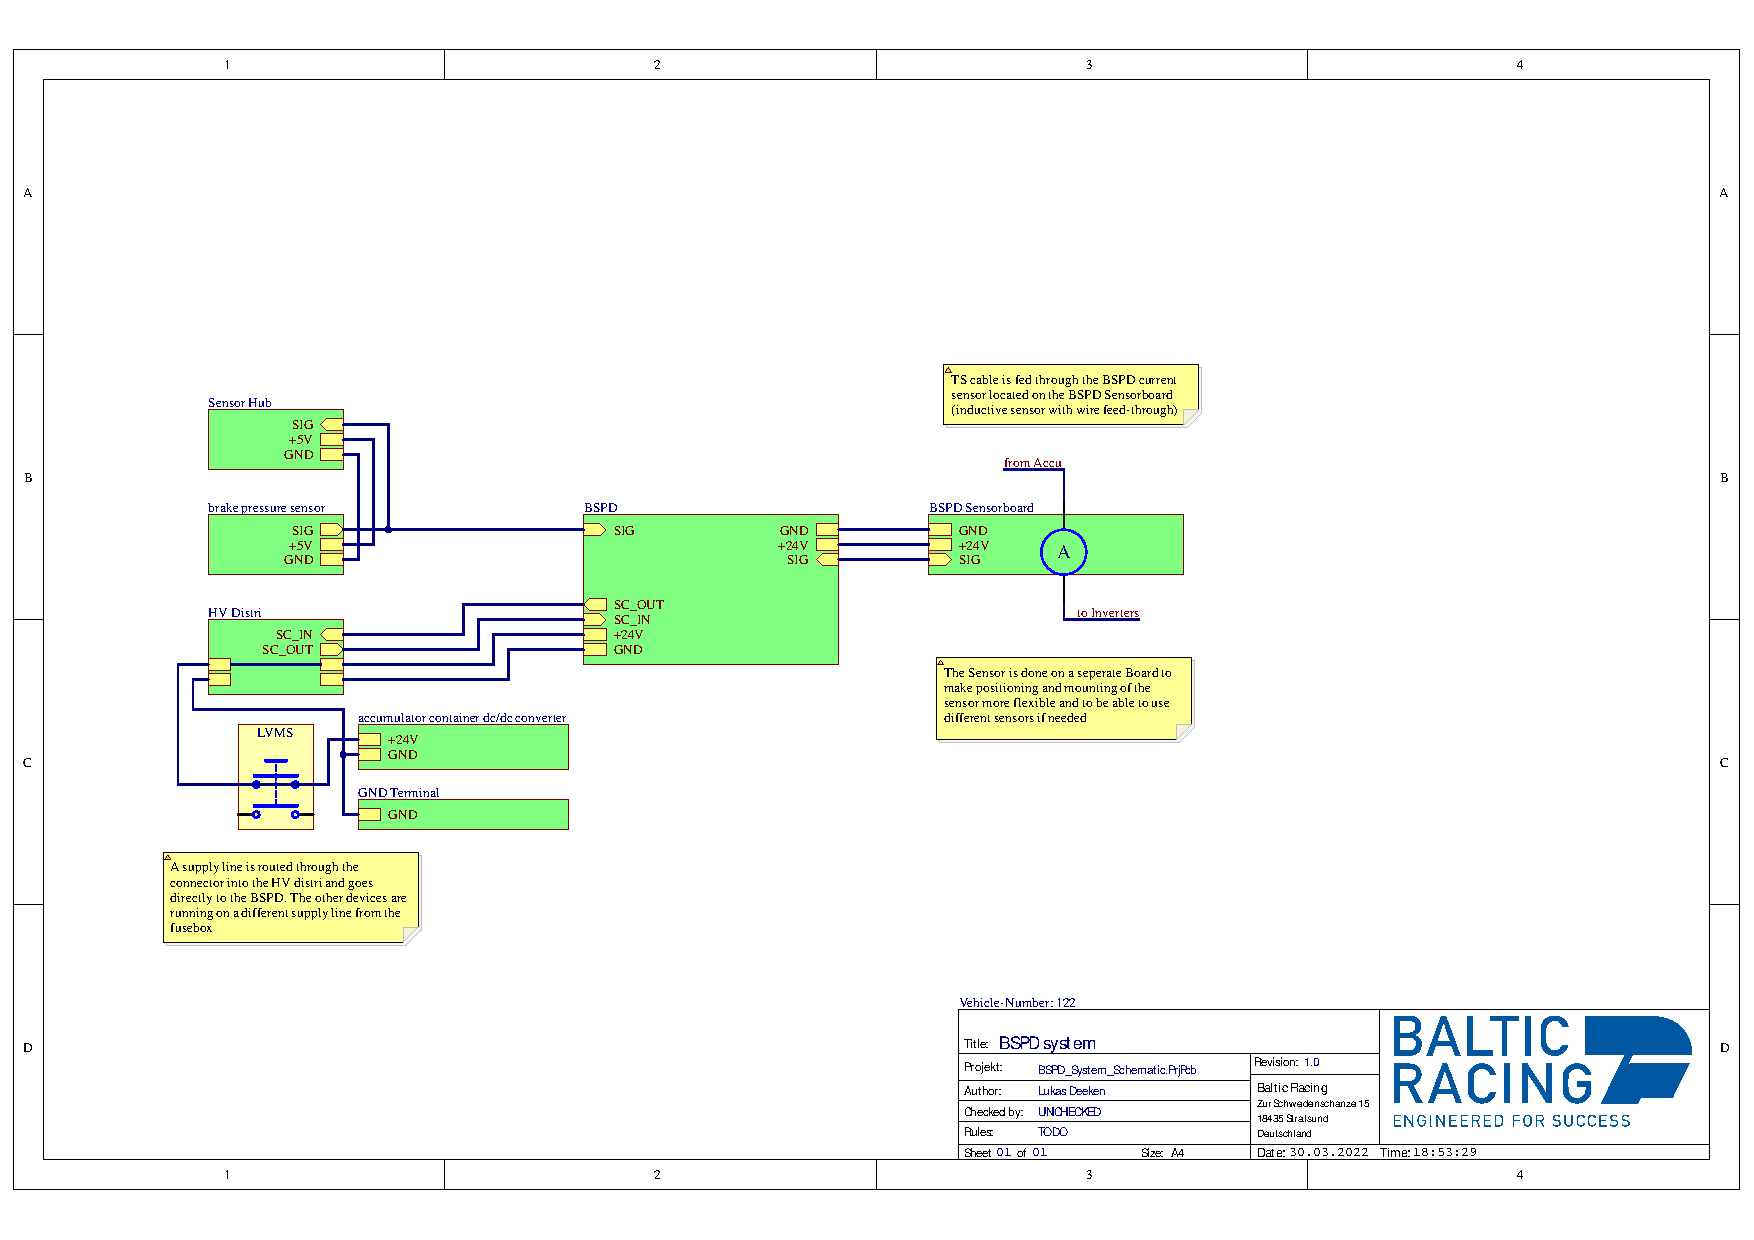
\includepdf[pages=-]{Schaltplaene/BSPD_Schematic_w_System_2.pdf}
\subsection{Chager}
\includepdf[pages=-]{Schaltplaene/Charger_Schematic_V3.pdf}
\subsection{\ac{HV}-DCDC}
\includepdf[pages=-]{Schaltplaene/HV_DCDC.pdf}
\subsection{HV-Distribution}
\includepdf[pages=-]{Schaltplaene/hv-distribution-board.pdf}
\subsection{\ac{SDC}}
\includepdf[pages=-]{Schaltplaene/Shutdowncircuit.pdf}
\subsection{\ac{TS}-System-Schematic}
\includepdf[pages=-]{Schaltplaene/Tractive_System_Schematic_V4.pdf}
\subsection{\ac{AMS}-Master}
\includepdf[pages=-]{Schaltplaene/tsac-distribution.pdf}
\subsection{\ac{TSAL}}
\includepdf[pages=-]{Schaltplaene/tsal.pdf}

	
	\chapter{Zweiter Anhang}
	Beispieltext
	
	%% ++++++++++++++++++++++++++++++++++++++++++++++++++++++++++++
%% Anhang: Beispielkapitel "Programm A"
%% ++++++++++++++++++++++++++++++++++++++++++++++++++++++++++++
%
%  Gerüst:
%  * Version 0.11
%  * Dipl.-Ing. Karsten Renhak, karsten.renhak@tu-ilmenau.de
%  * Fachgebiet Kommunikationsnetze, TU Ilmenau
%
%  Für Hauptseminare, Studienarbeiten, Diplomarbeiten
%
%  Autor           : Max Mustermann
%  Letzte Änderung : 31.12.2011
%

\section{ESF}
\includepdf[pages=-]{Schaltplaene/FSE22_ESF_DE_Stralsund_UAS_Car122_V1.1.pdf}
	\input{anhang2_2.tex}
		
	% Literaturverzeichnis einbinden
	\input{anhang_literaturverzeichnis.tex}
	
\end{document}

